\chapter{Results}
%Looking also at the general picture usually helps, for example, looking at figure \ref{heatmap}, it is clear that way more paths ended up hitting the lights on the ceiling and on the staircase rather than the two light portals down the hall

Assessing the validity of a tool without performing user tests is often pointless but, due to the complexity of the tool, there was no time to perform any. In their absence, the analysis of two couples of significant datasets are presented.

\section{Couple \#1}

\section{Couple \#2}

\begin{figure}
	\centering
	\begin{subfigure}[t]{0.32\linewidth}
		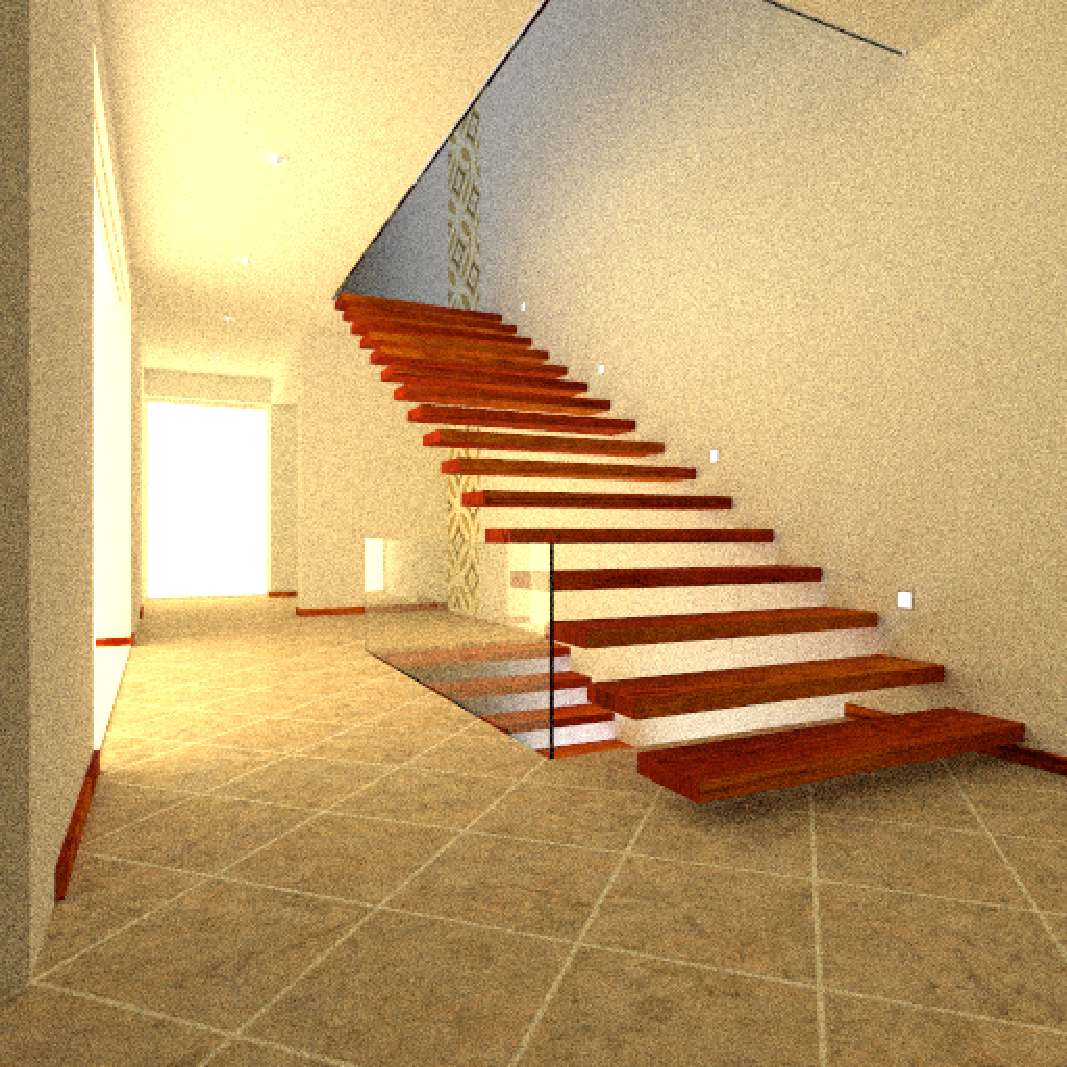
\includegraphics[width=\textwidth]{chapters/chapter_results/correctrender2}
		\caption{Render \texttt{A}}
	\end{subfigure}
	\begin{subfigure}[t]{0.32\linewidth}
		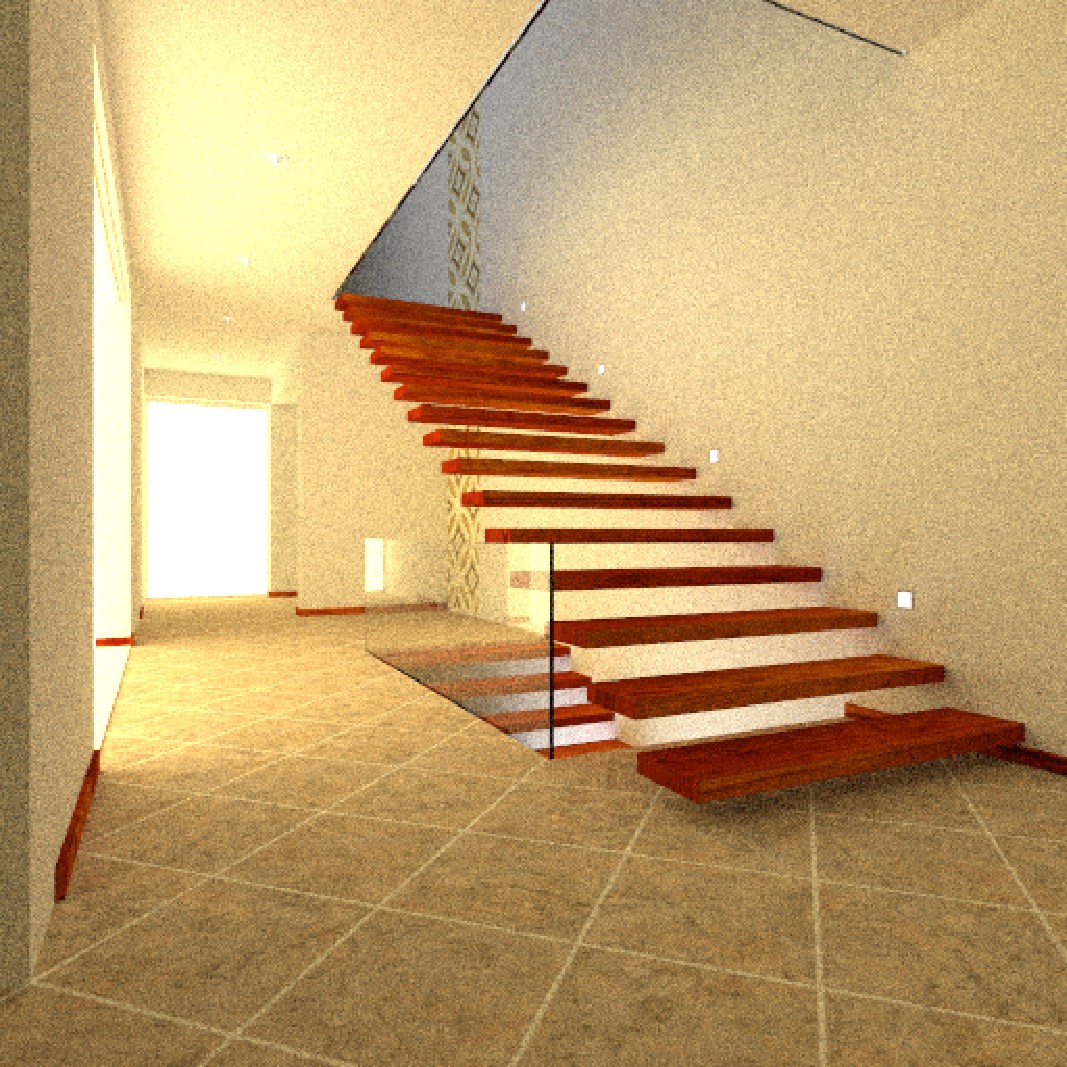
\includegraphics[width=\textwidth]{chapters/chapter_results/wrongrender2}
		\caption{Render \texttt{B}}
	\end{subfigure}
	\begin{subfigure}[t]{0.32\linewidth}
		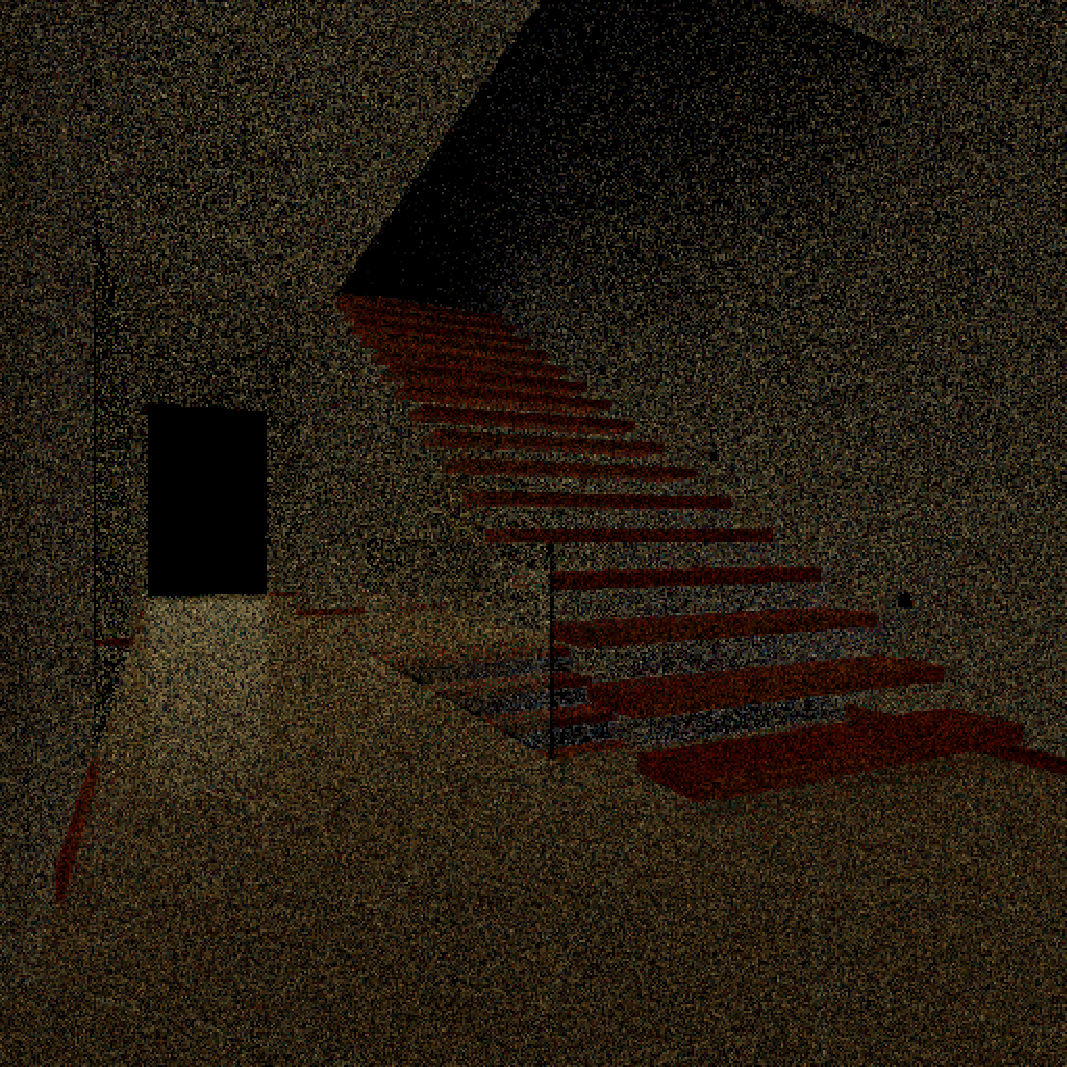
\includegraphics[width=\textwidth]{chapters/chapter_results/render2difference}
		\caption{\texttt{A} $-$ \texttt{B}}
		\label{render2difference}
	\end{subfigure}

	\caption{Render images of the two datasets (\textbf{a}, \textbf{b}) and their mathematical delta (\textbf{c}) to show their differences. (\textbf{c}) has been generated outside the tool and presented for clarity.}
	\label{couple2render}
\end{figure}

To provide a more challenging test, the datasets of which renders are shown in figure \ref{couple2render}, both generated by the na\"ive tracer of Yocto/GL \cite{pellacini2019yocto}, have been tinkered to present a very subtle difference. Dataset \texttt{A} is correct while dataset \texttt{B} has been generated after introducing an error in the sampling of microfacet distributions: the direction vector generated according to the distribution has the \textit{y} and \textit{z} components swapped before being transformed from surface space to world space. Logically, this should have generated way more noticeable visual artifacts in the render but, as highlighted by figure \ref{render2difference}, it looks like the wrong render does not account for the Fresnel effect correctly. By just looking at the renders, the user might be led into thinking that there is an error in the Fresnel term calculation or in the surface material in general but here, the situation is different: the direction of the rays are wrong not the calculations of the energy they carry.


\begin{figure}
	\centering
	\begin{subfigure}[t]{0.24\linewidth}
		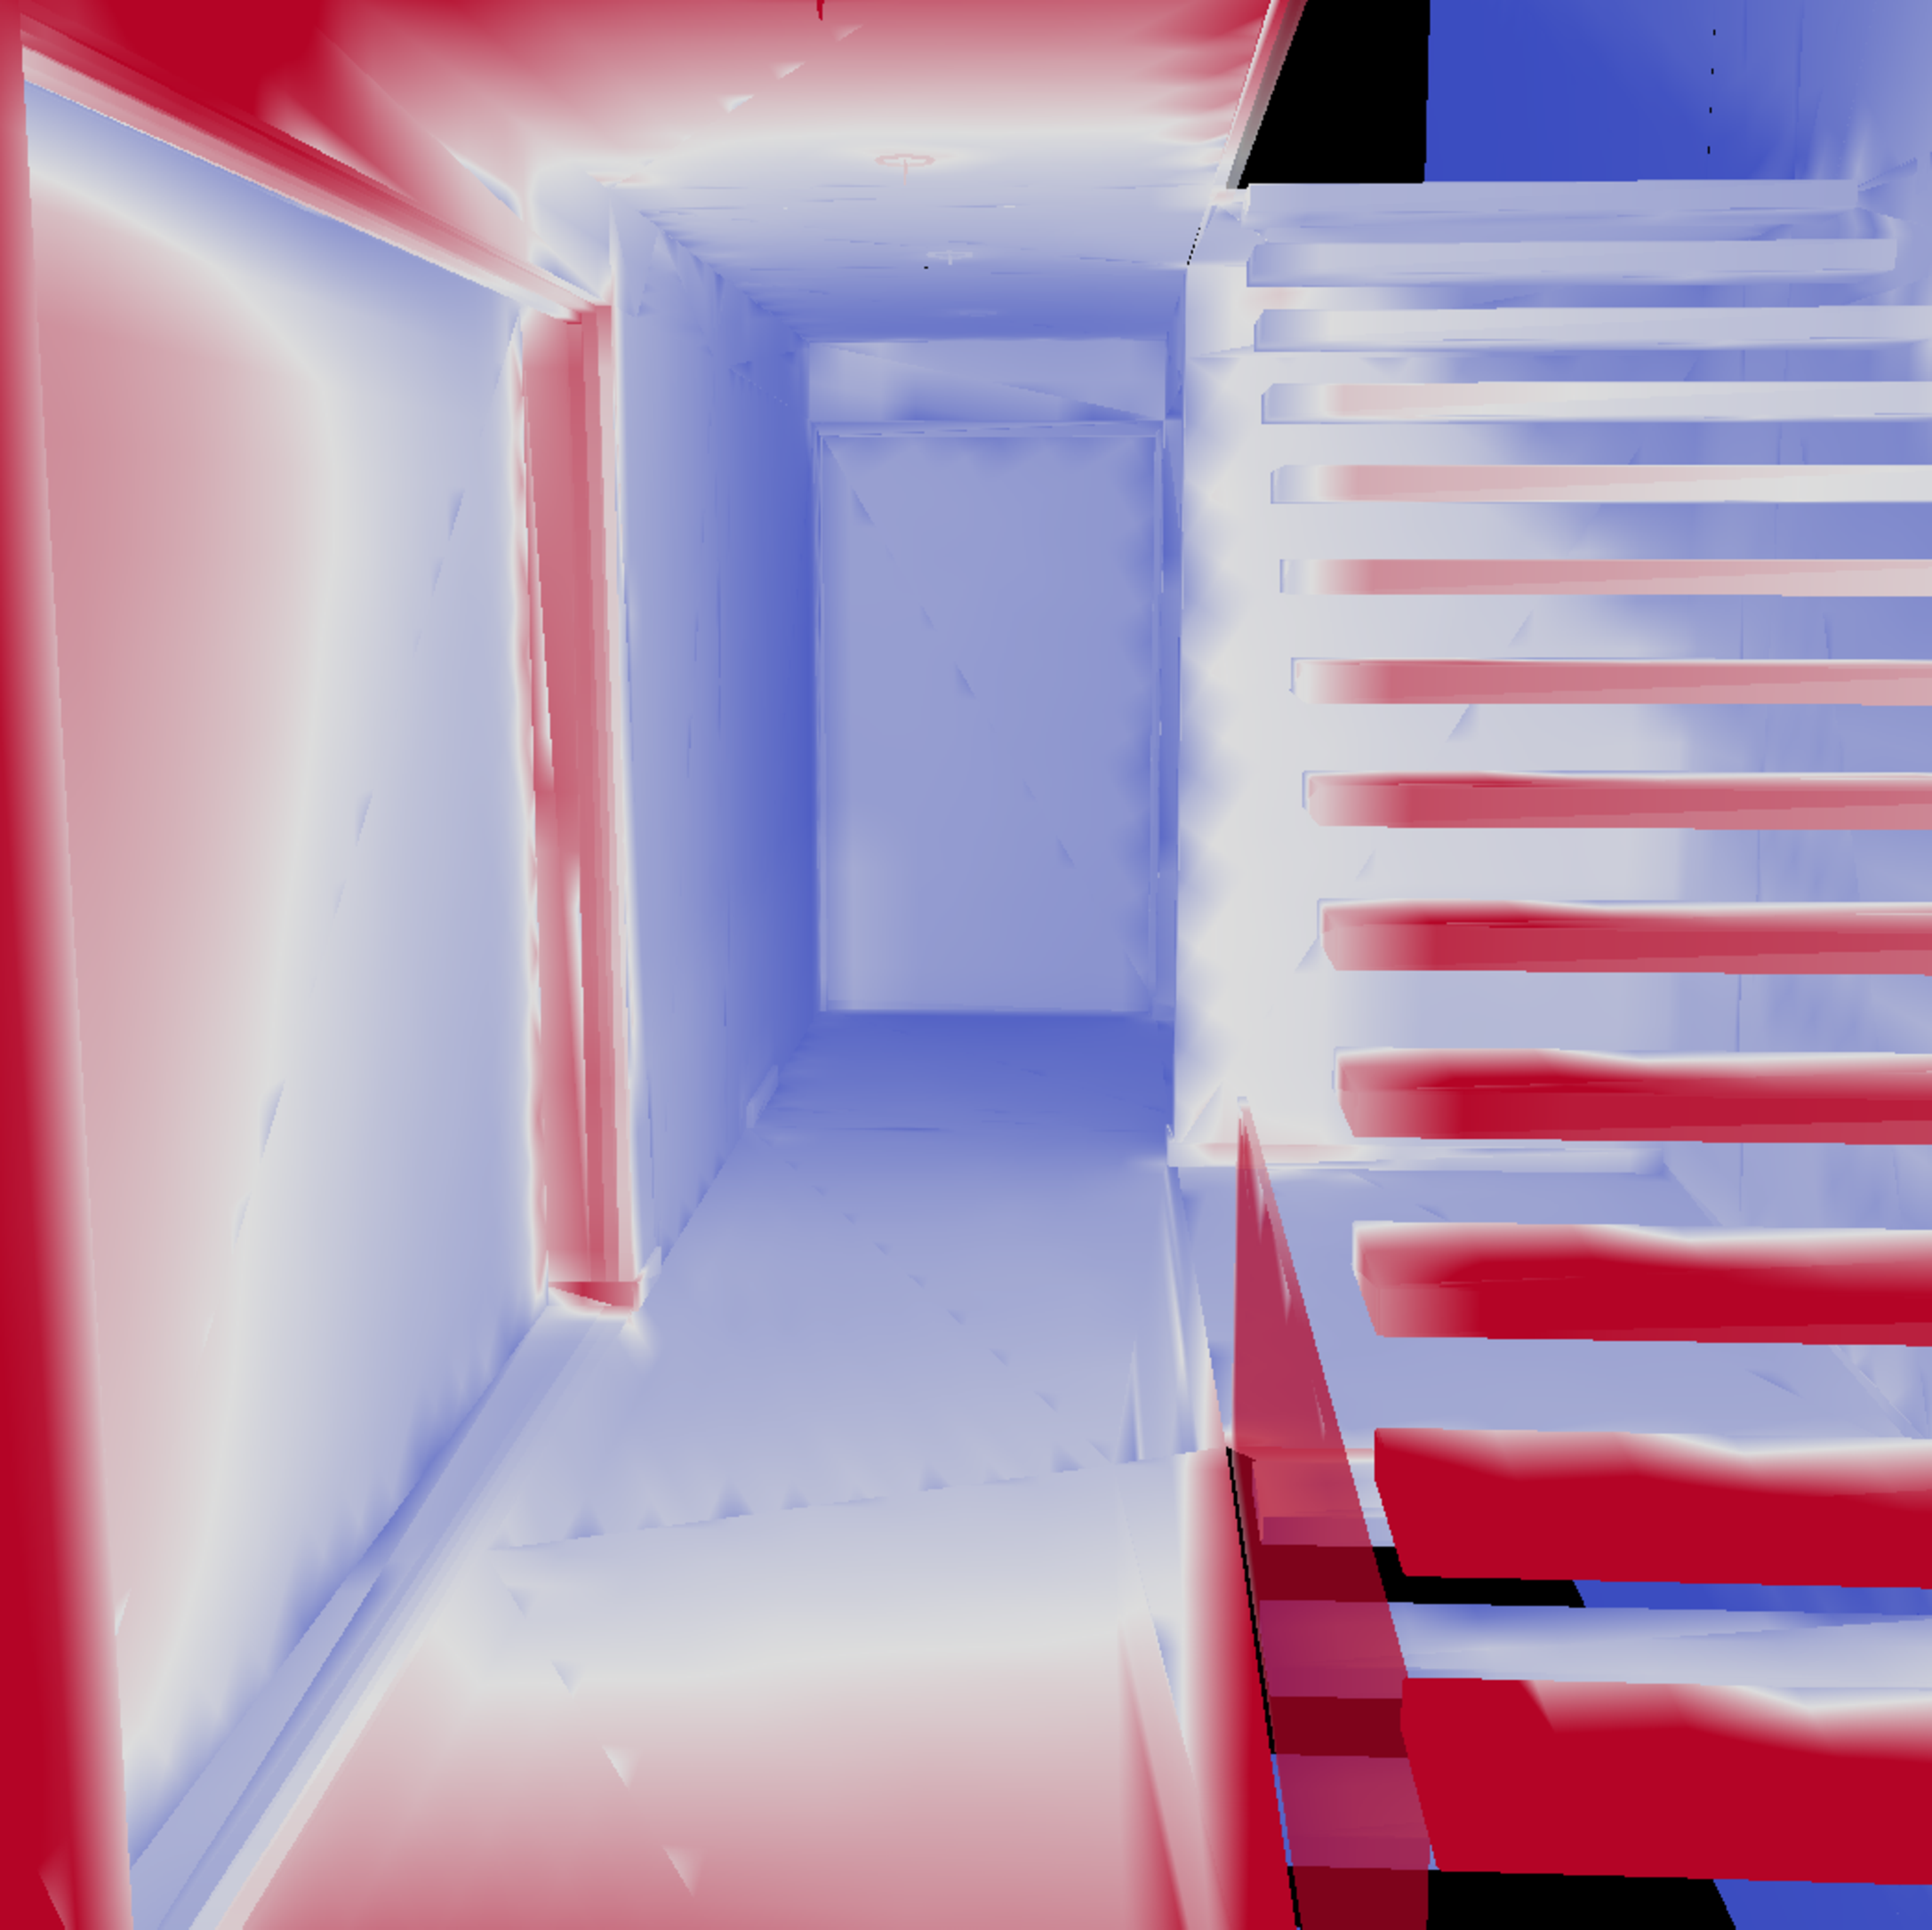
\includegraphics[width=\textwidth]{chapters/chapter_results/correct2heatmap1}
		\caption{Dataset \texttt{A} heatmap 1}
	\end{subfigure}
	\begin{subfigure}[t]{0.24\linewidth}
		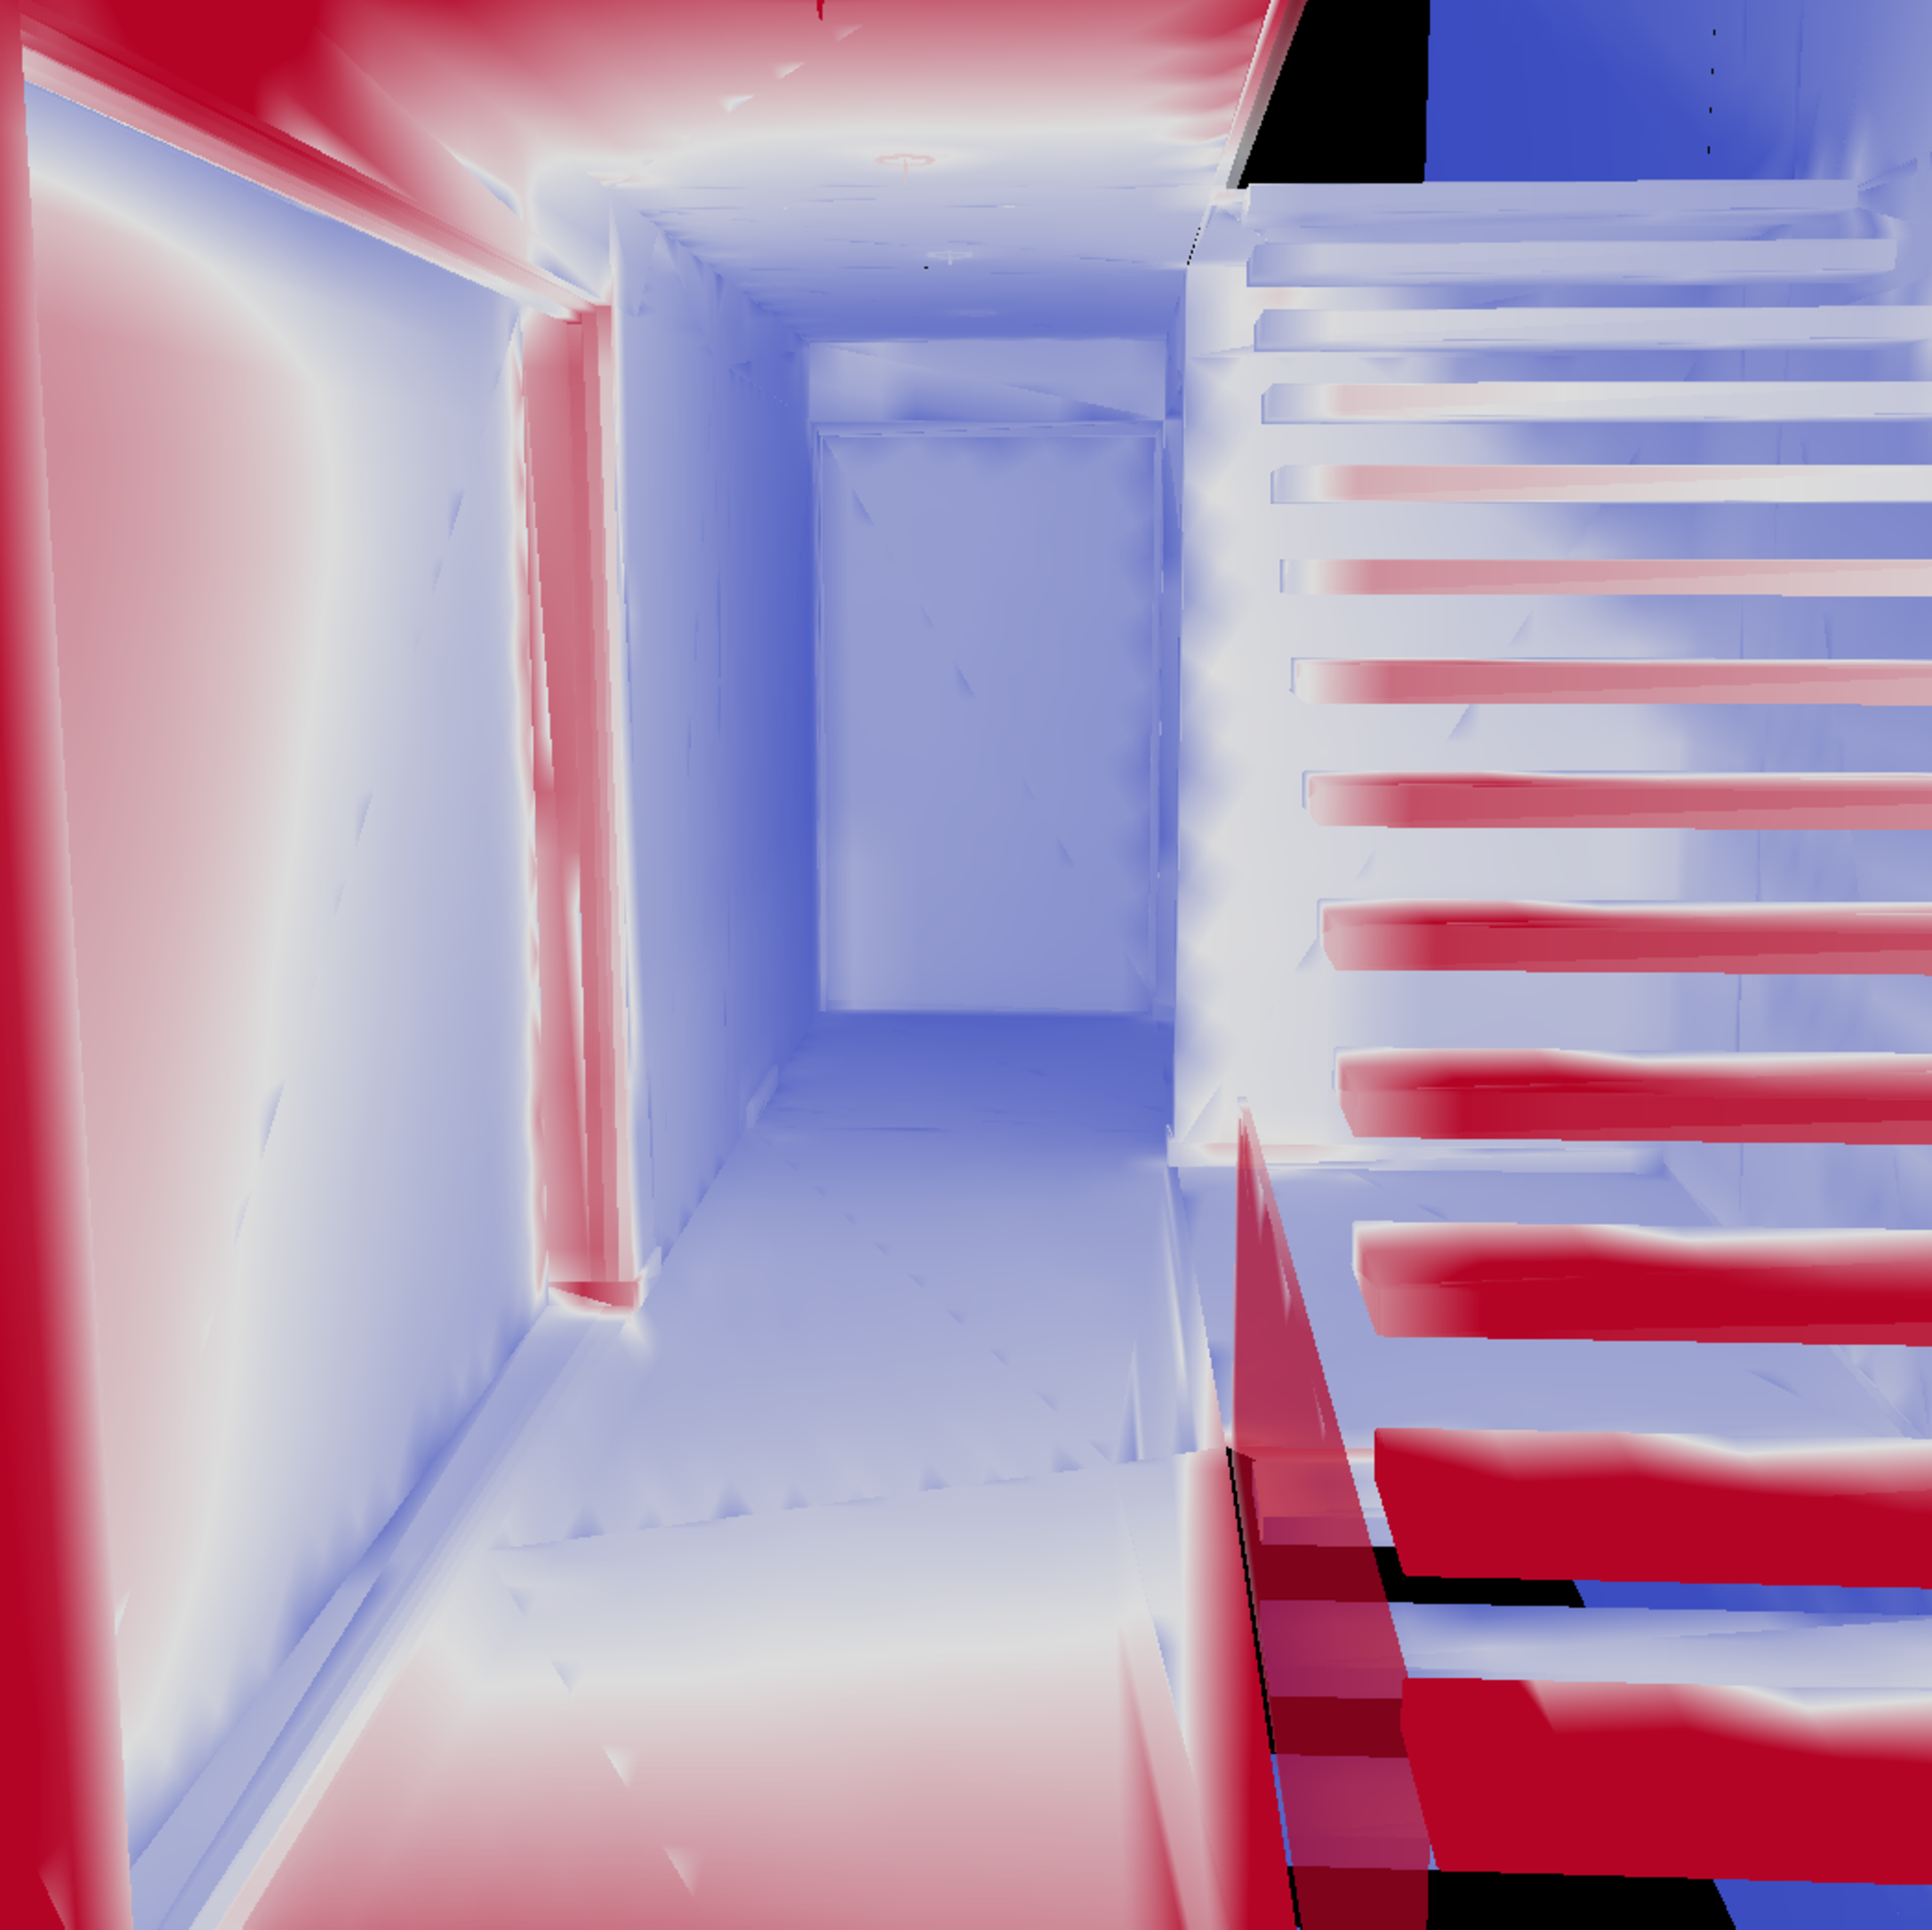
\includegraphics[width=\textwidth]{chapters/chapter_results/wrong2heatmap1}
		\caption{Dataset \texttt{B} heatmap 1}
	\end{subfigure}
	\begin{subfigure}[t]{0.24\linewidth}
		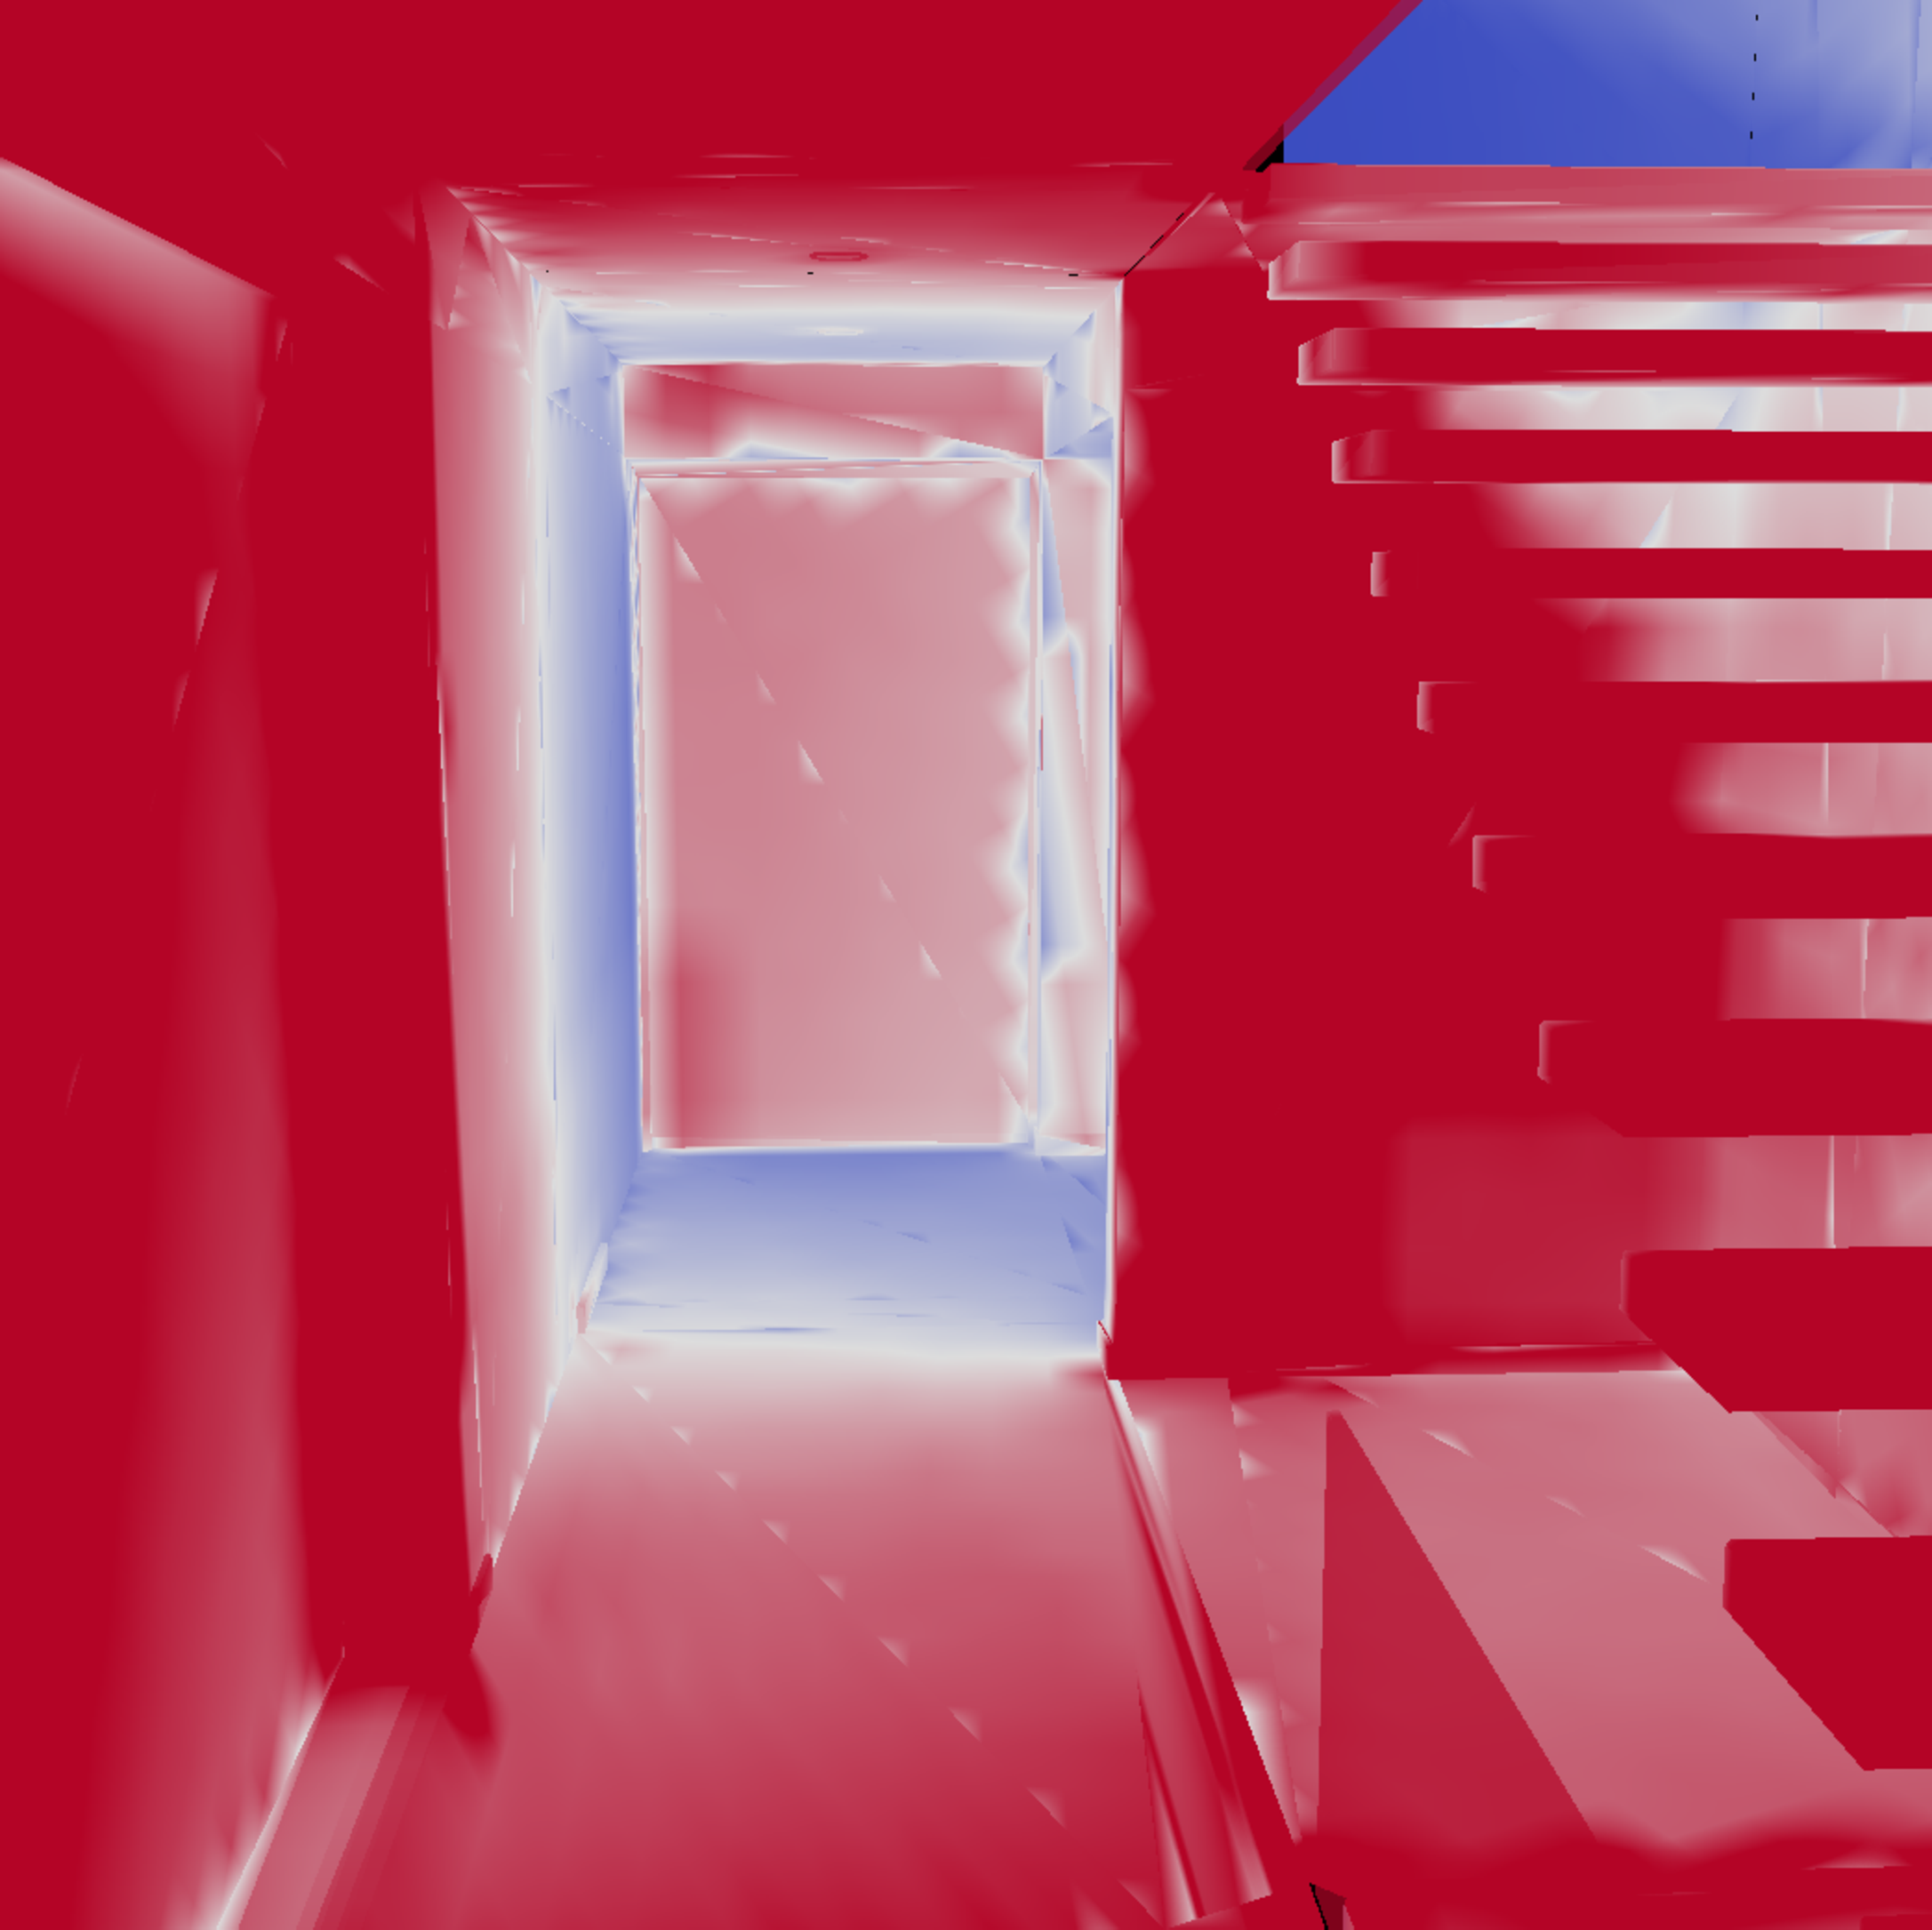
\includegraphics[width=\textwidth]{chapters/chapter_results/correct2heatmap2}
		\caption{Dataset \texttt{A} heatmap 2}
	\end{subfigure}
	\begin{subfigure}[t]{0.24\linewidth}
		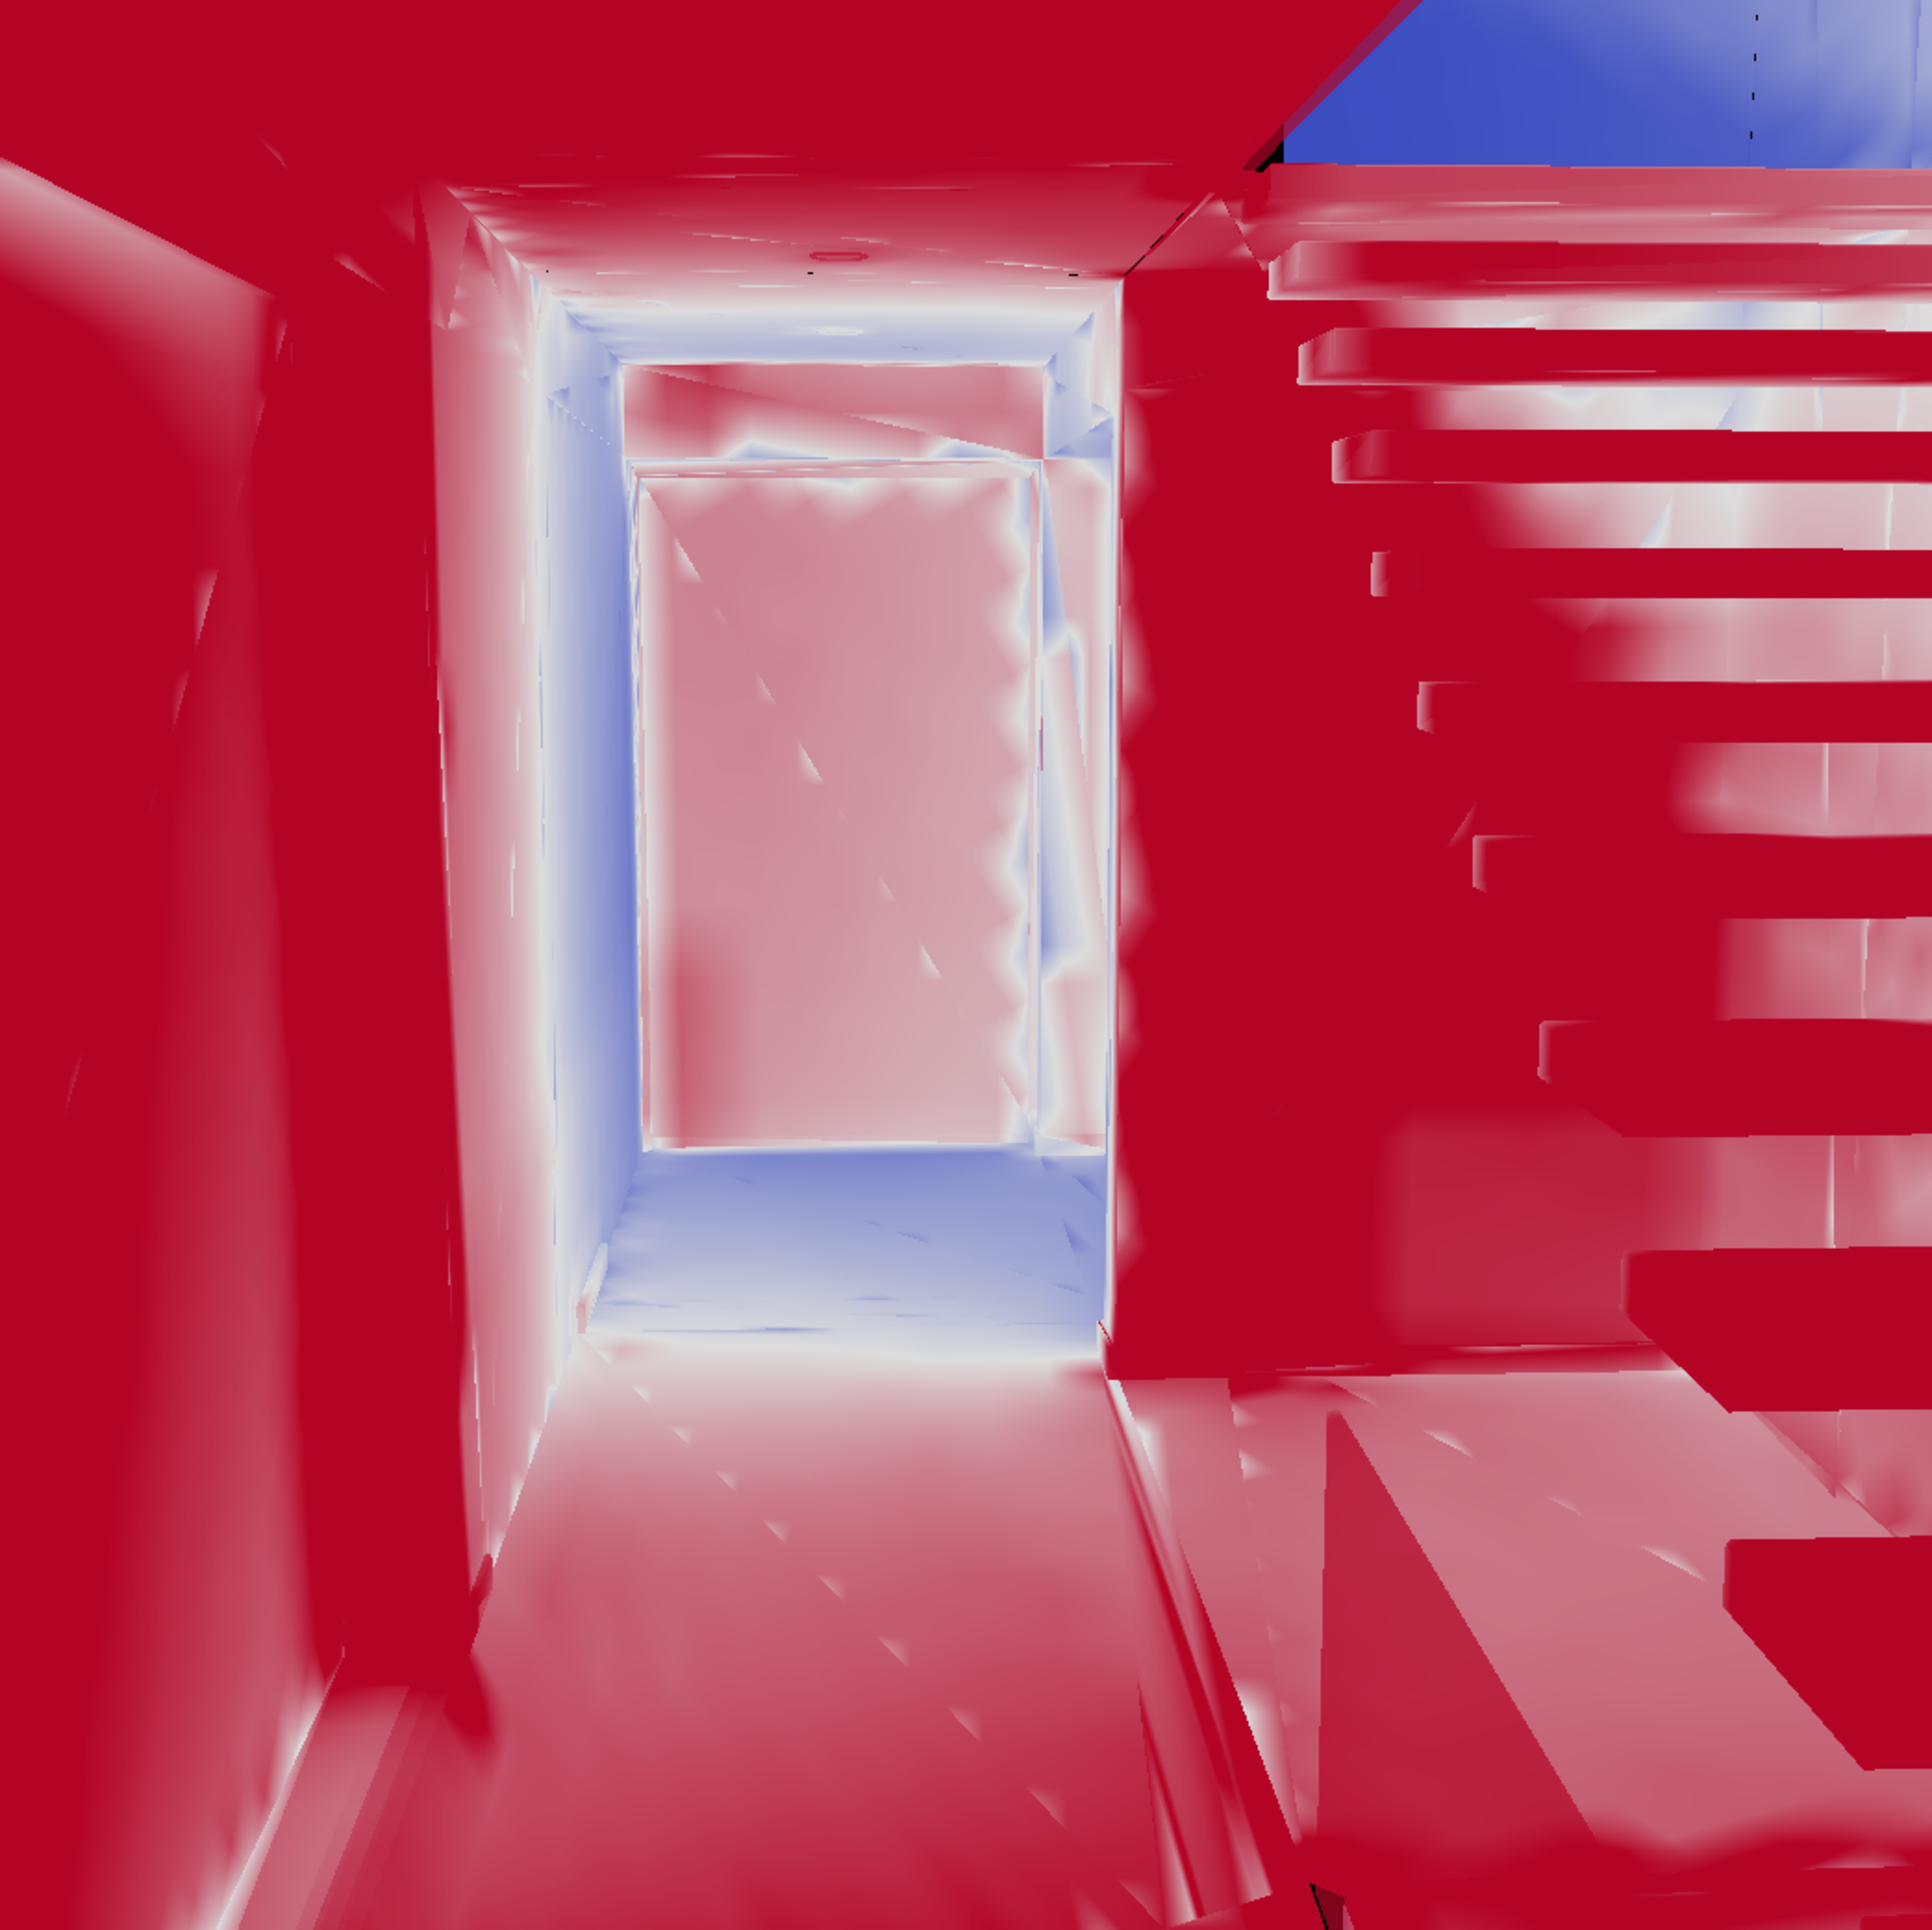
\includegraphics[width=\textwidth]{chapters/chapter_results/wrong2heatmap2}
		\caption{Dataset \texttt{B} heatmap 2}
	\end{subfigure}

	\caption{Heatmap renderings for both datasets from two different cameras and with two different parameters for the \textbf{“Heatmap max”} parameter (for (\textbf{a}) and (\textbf{b}) is set to $100,000$ while for (\textbf{c}) and (\textbf{d}) is set to $40,000$).}
	\label{couple2heatmaps}
\end{figure}

The first instinct was to check the heatmap on the areas where the renders are most different --- that is to say the floor right in front of the light portal at the end of the corridor --- but only minimal differences can be spotted. In the screenshots in figure \ref{couple2heatmaps} vague changes can be seen with a lot of effort, and they just achieve to communicate that the correct dataset --- dataset \texttt{A} --- has a slightly higher bounces density than the wrong dataset. No conclusions can be deducted from this little information.

\begin{figure}
	\centering
	\begin{subfigure}[t]{0.32\linewidth}
		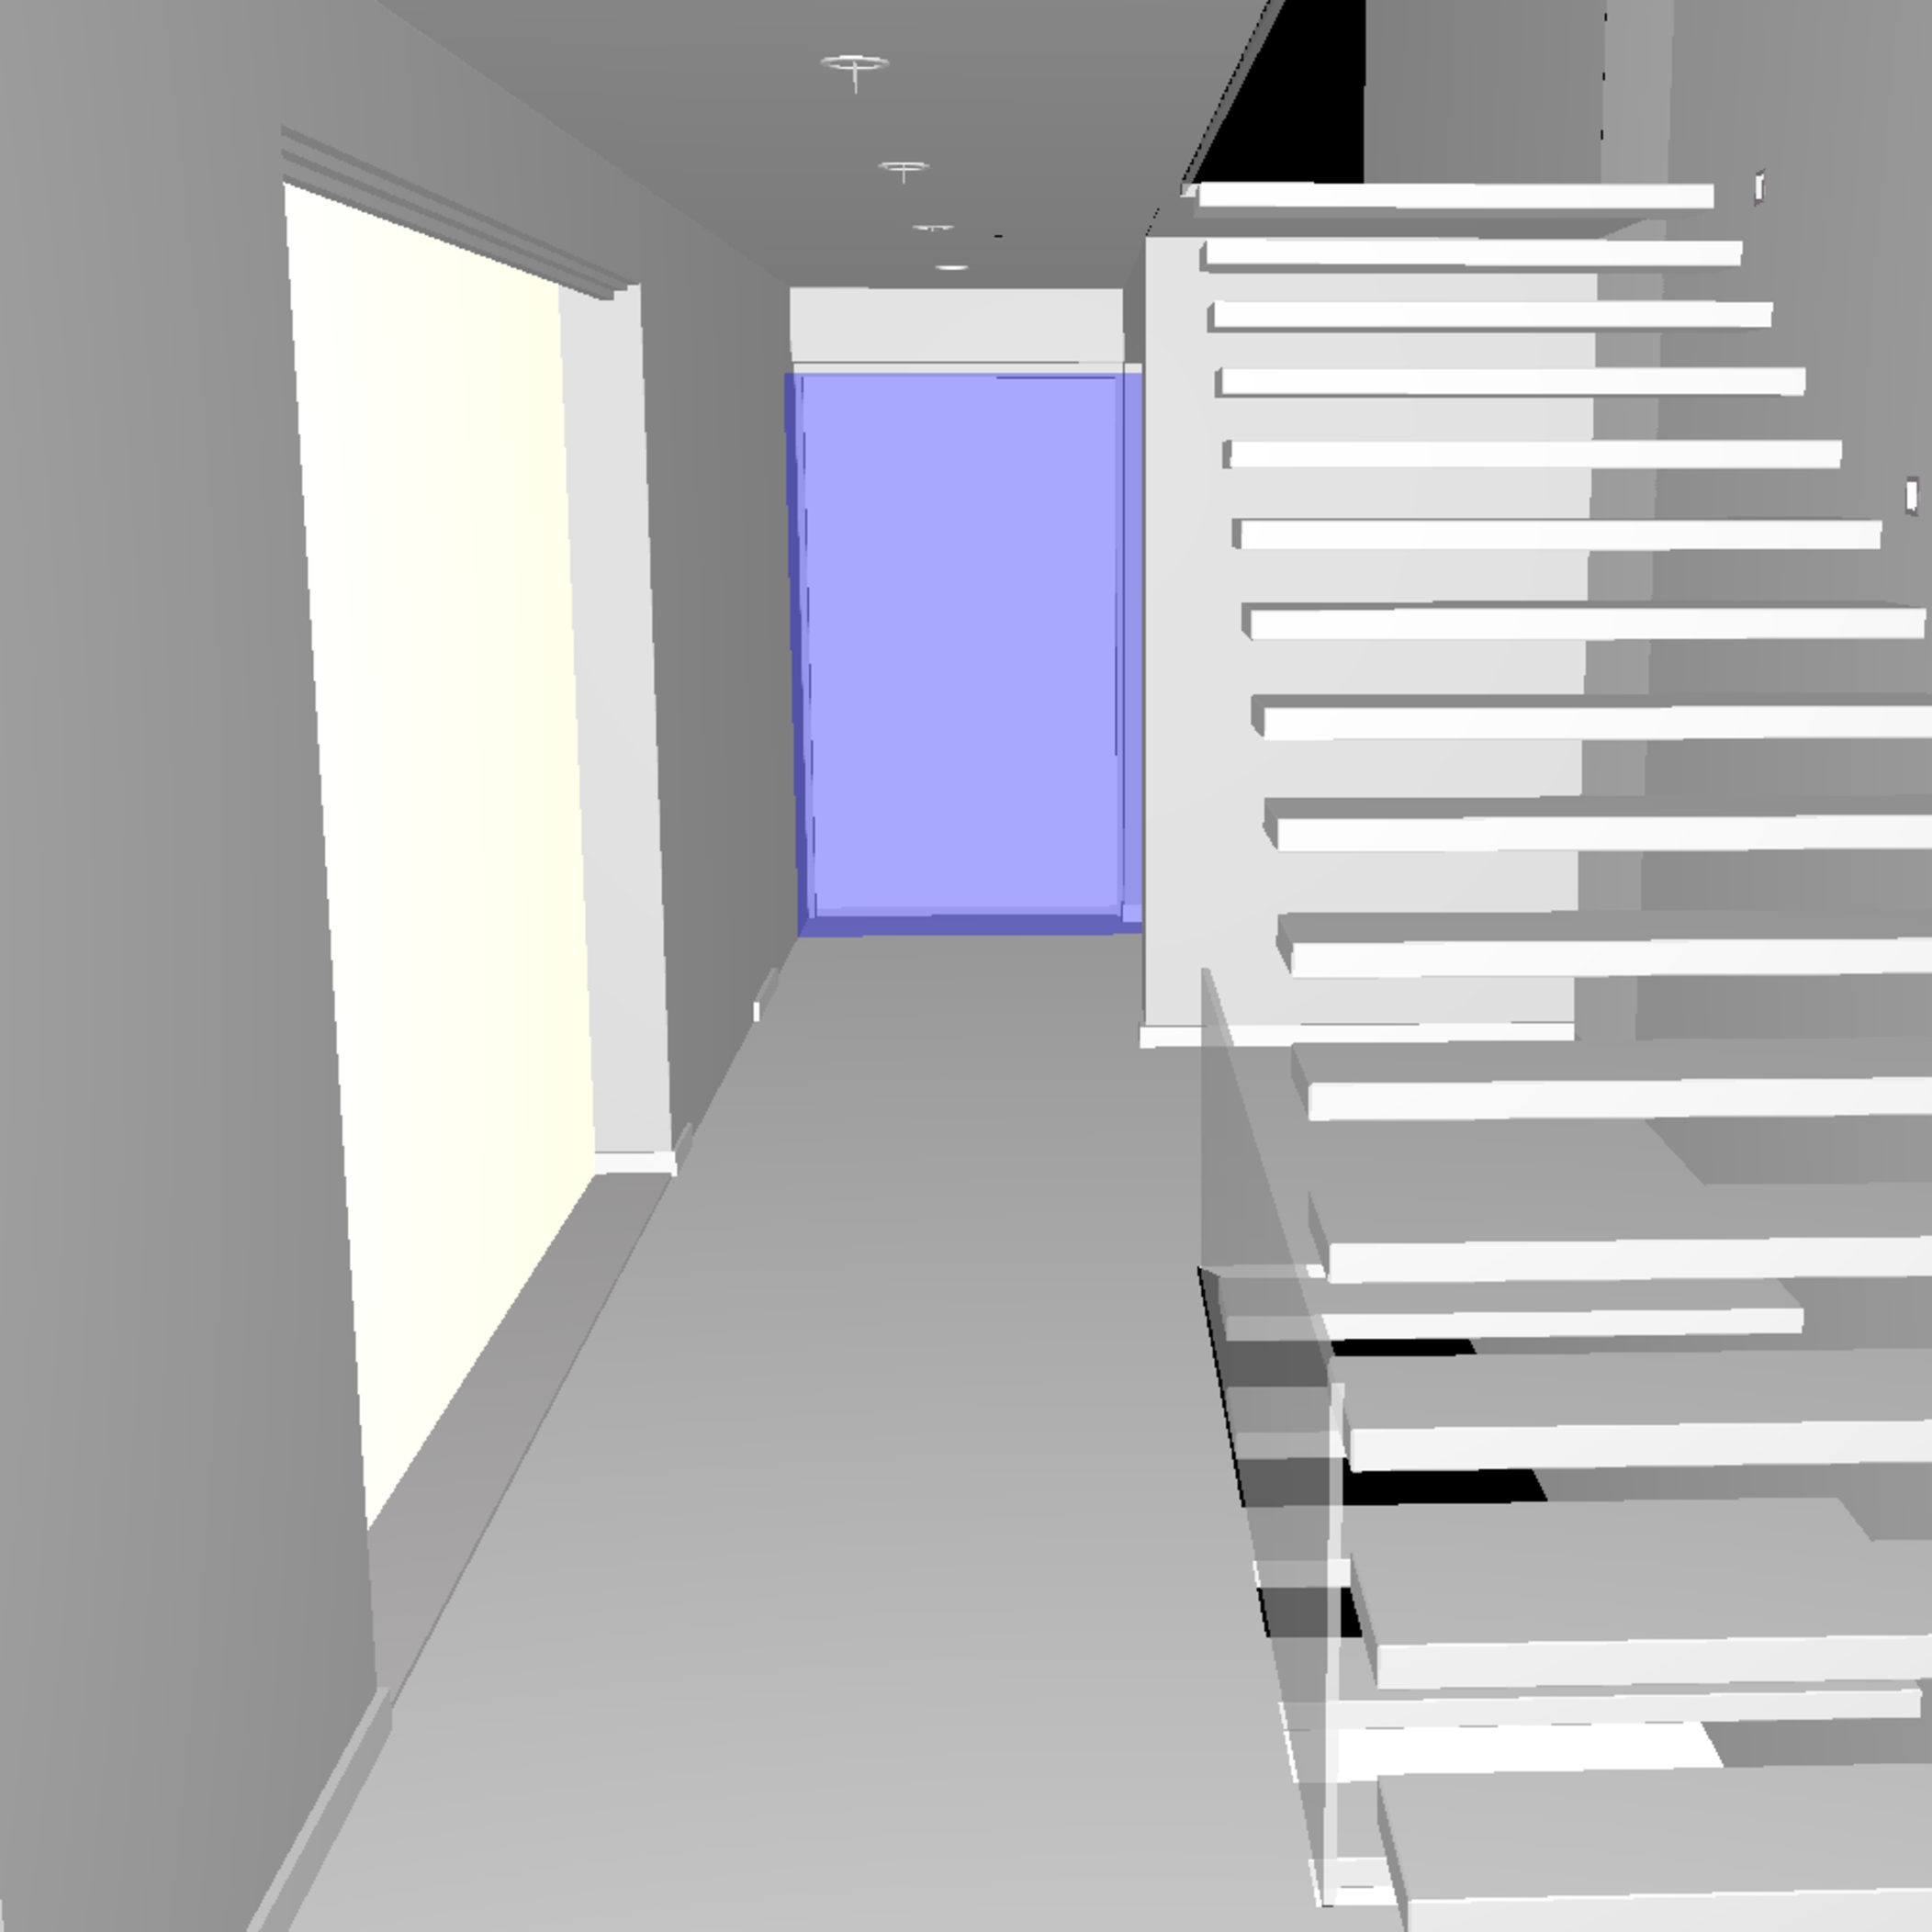
\includegraphics[width=\textwidth]{chapters/chapter_results/ds2filterpos1}
		\caption{Filter position}
	\end{subfigure}
	\begin{subfigure}[t]{0.32\linewidth}
		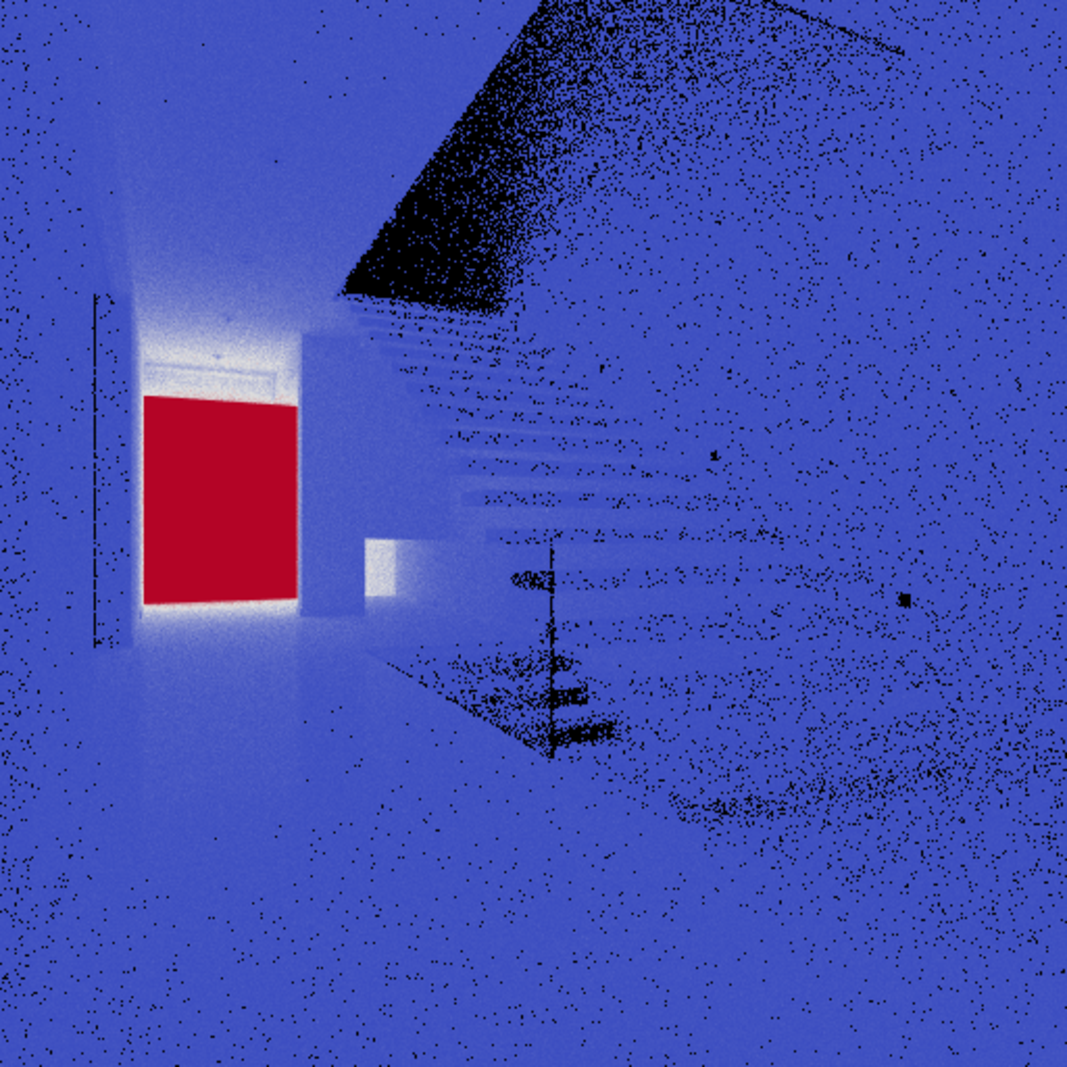
\includegraphics[width=\textwidth]{chapters/chapter_results/correct2ppp}
		\caption{Dataset \texttt{A}}
		\label{correct2ppp}
	\end{subfigure}
	\begin{subfigure}[t]{0.32\linewidth}
		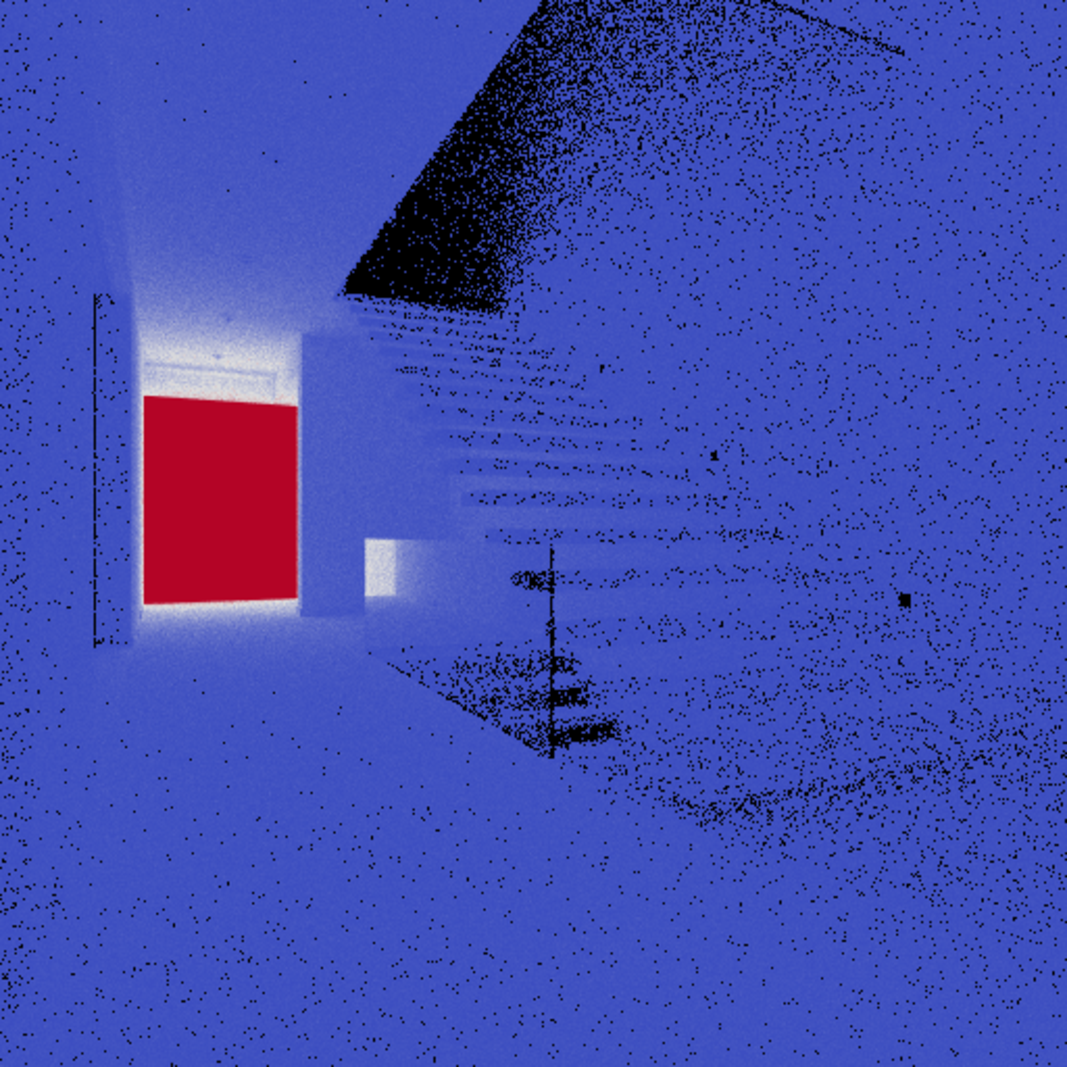
\includegraphics[width=\textwidth]{chapters/chapter_results/wrong2ppp}
		\caption{Dataset \texttt{B}}
		\label{wrong2ppp}
	\end{subfigure}

	\caption{Paths per pixel visualization for the window filter shown in (\textbf{a}).}
	\label{couple2ppp}
\end{figure}

Next step has been to place a window filter covering the entirety of the light at the end of the corridor. Due to the high number of paths selected, the viewport was too visually cluttered to be of any utility, so the focus went on the \textbf{“Render”} panel in the \textbf{“Paths per pixel”} render mode. This, pictured in figures \ref{correct2ppp} and \ref{wrong2ppp}, showed how many more paths in dataset \texttt{A} having their first bounce of the floor ended up hitting that light. It seemed like a further confirmation that something was wrong with the Fresnel term computation.

\begin{figure}
	\centering
	\begin{subfigure}[t]{0.24\linewidth}
		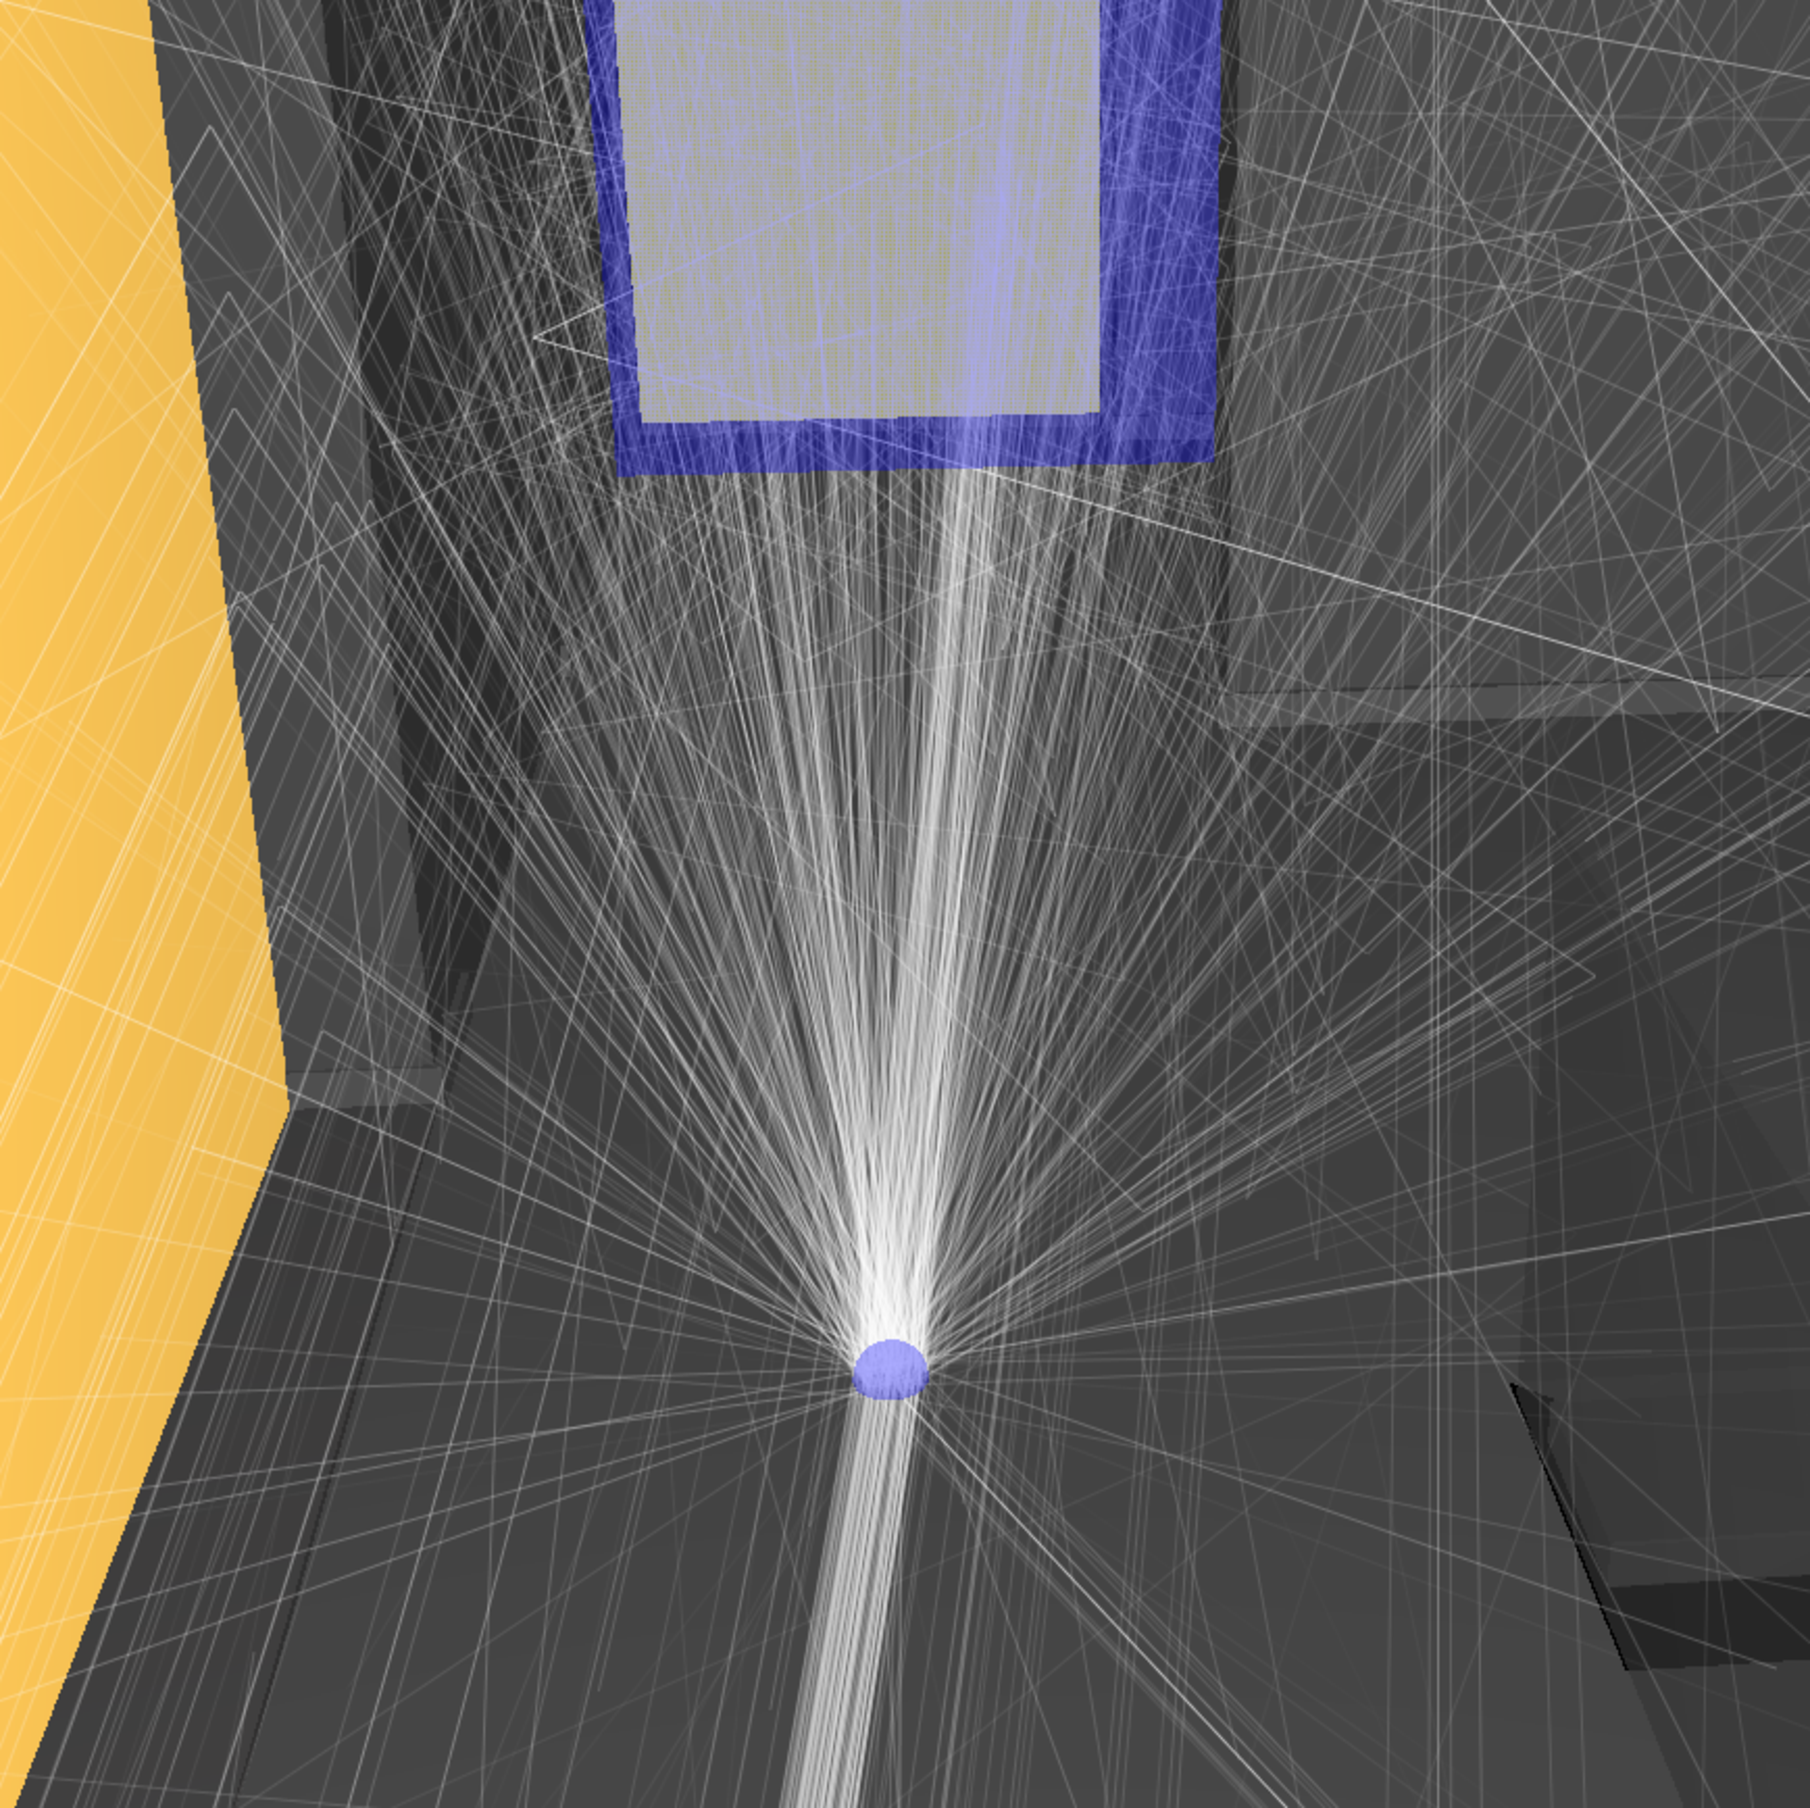
\includegraphics[width=\textwidth]{chapters/chapter_results/correct2pathsscaled}
		\caption{\texttt{A}, radiance scaled}
		\label{correct2pathsscaled}
	\end{subfigure}
	\begin{subfigure}[t]{0.24\linewidth}
		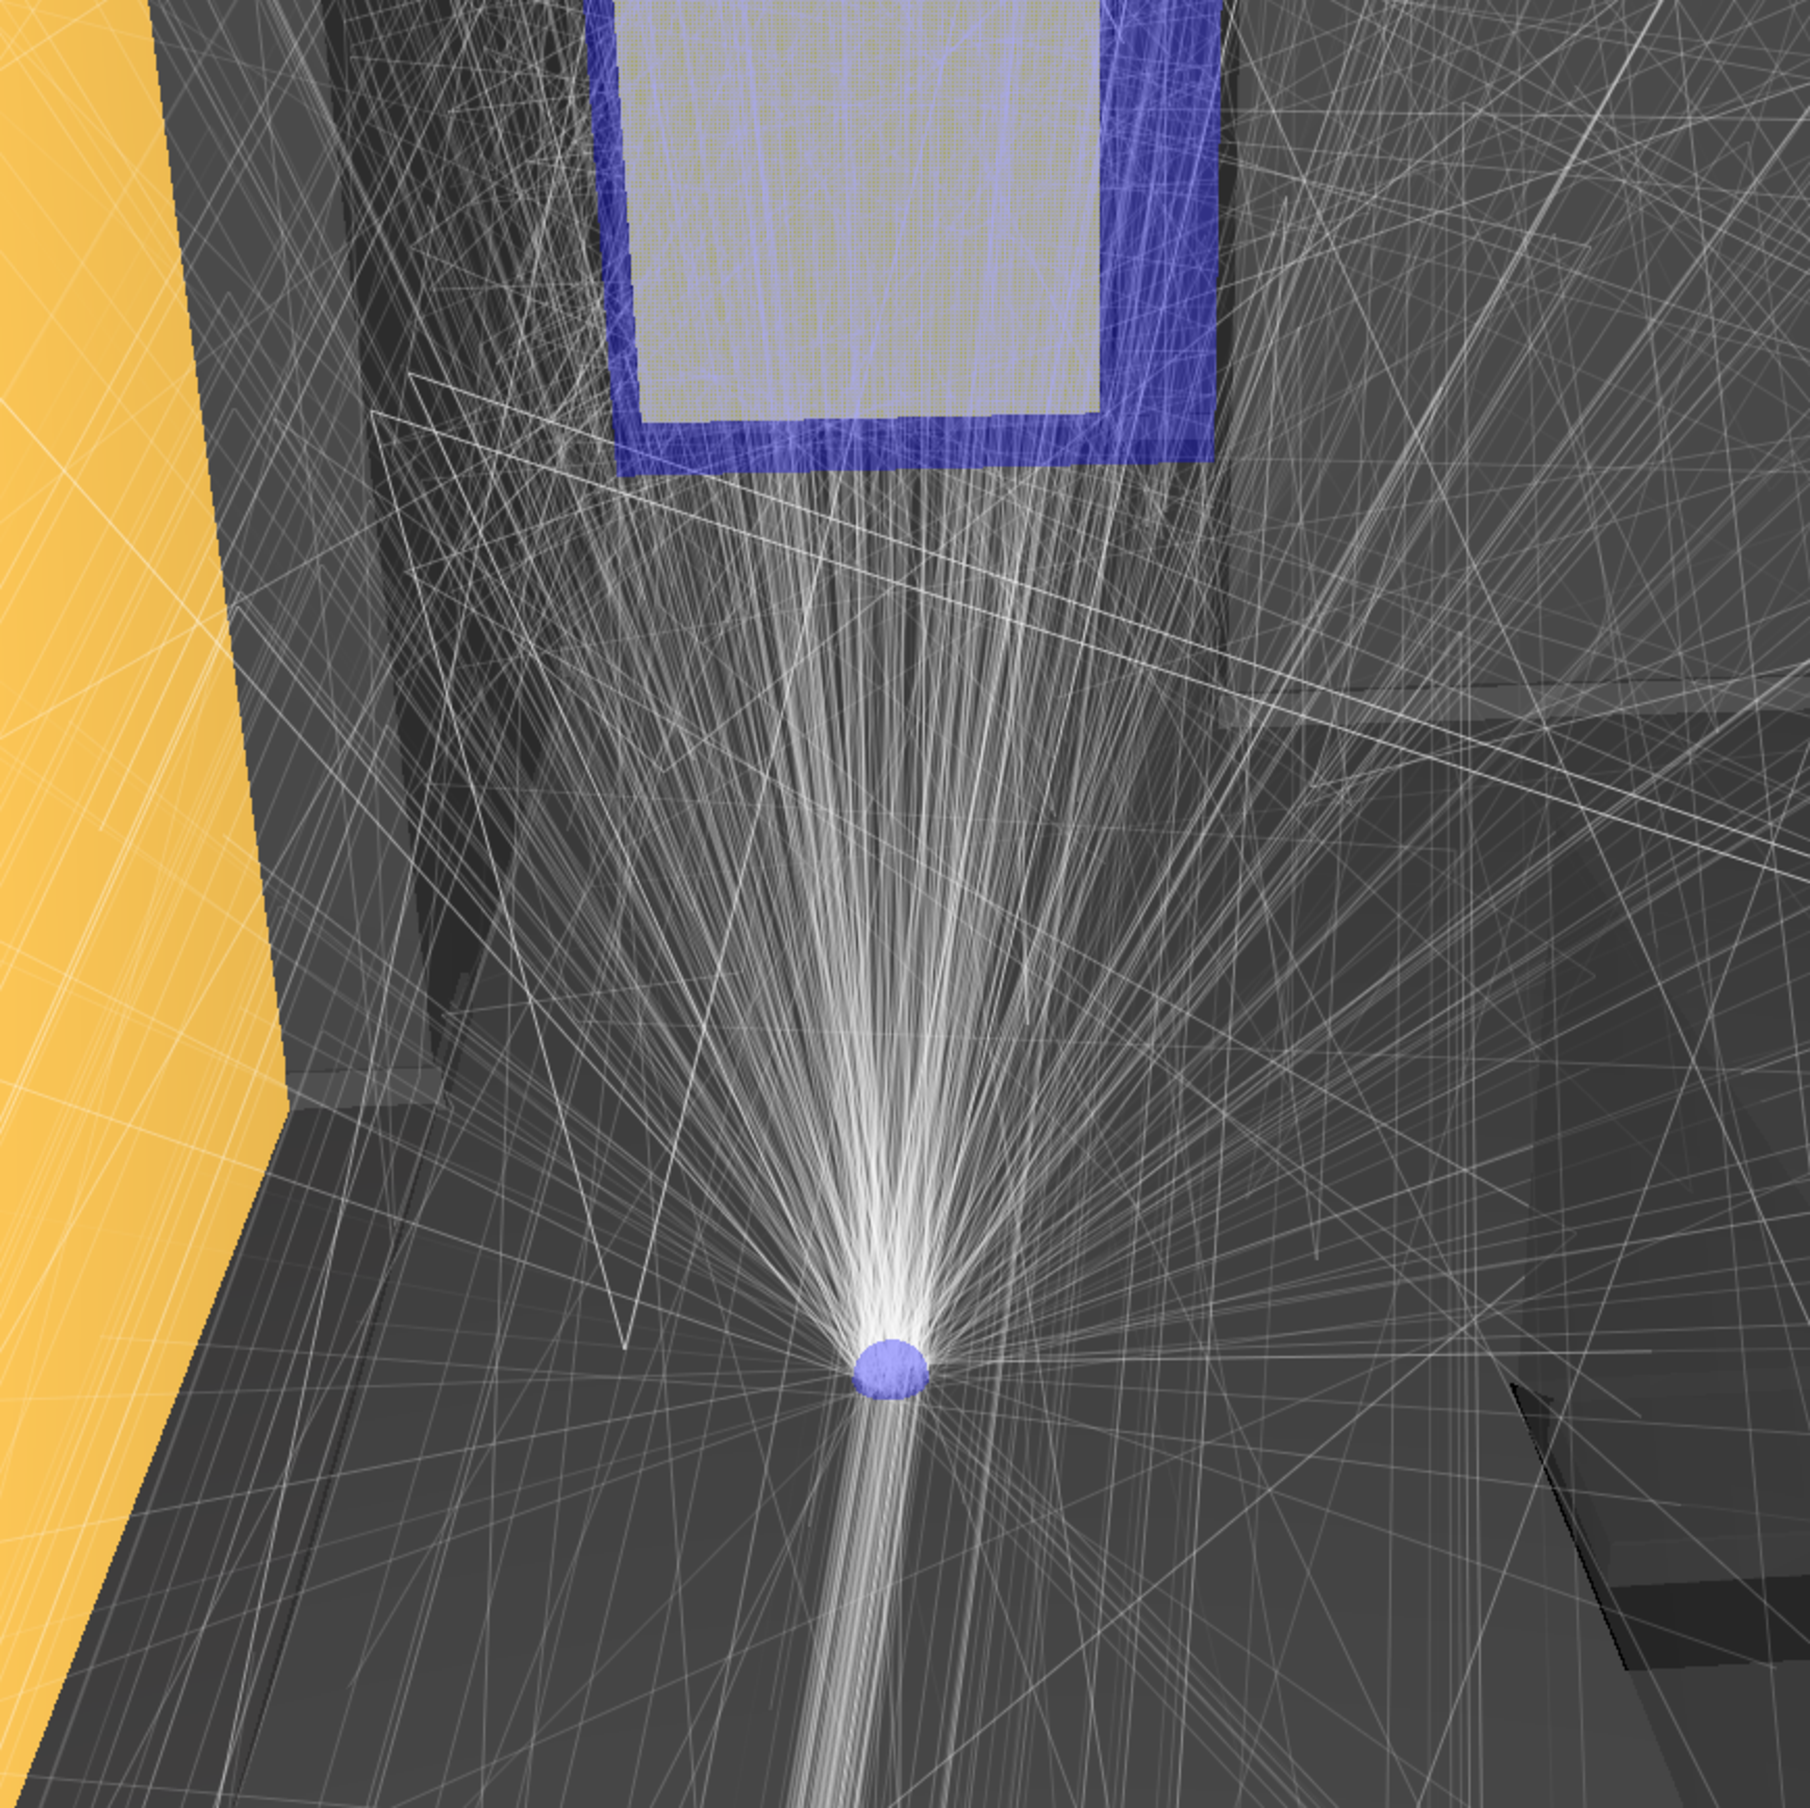
\includegraphics[width=\textwidth]{chapters/chapter_results/wrong2pathsscaled}
		\caption{\texttt{B}, radiance scaled}
		\label{wrong2pathsscaled}
	\end{subfigure}
	\begin{subfigure}[t]{0.24\linewidth}
		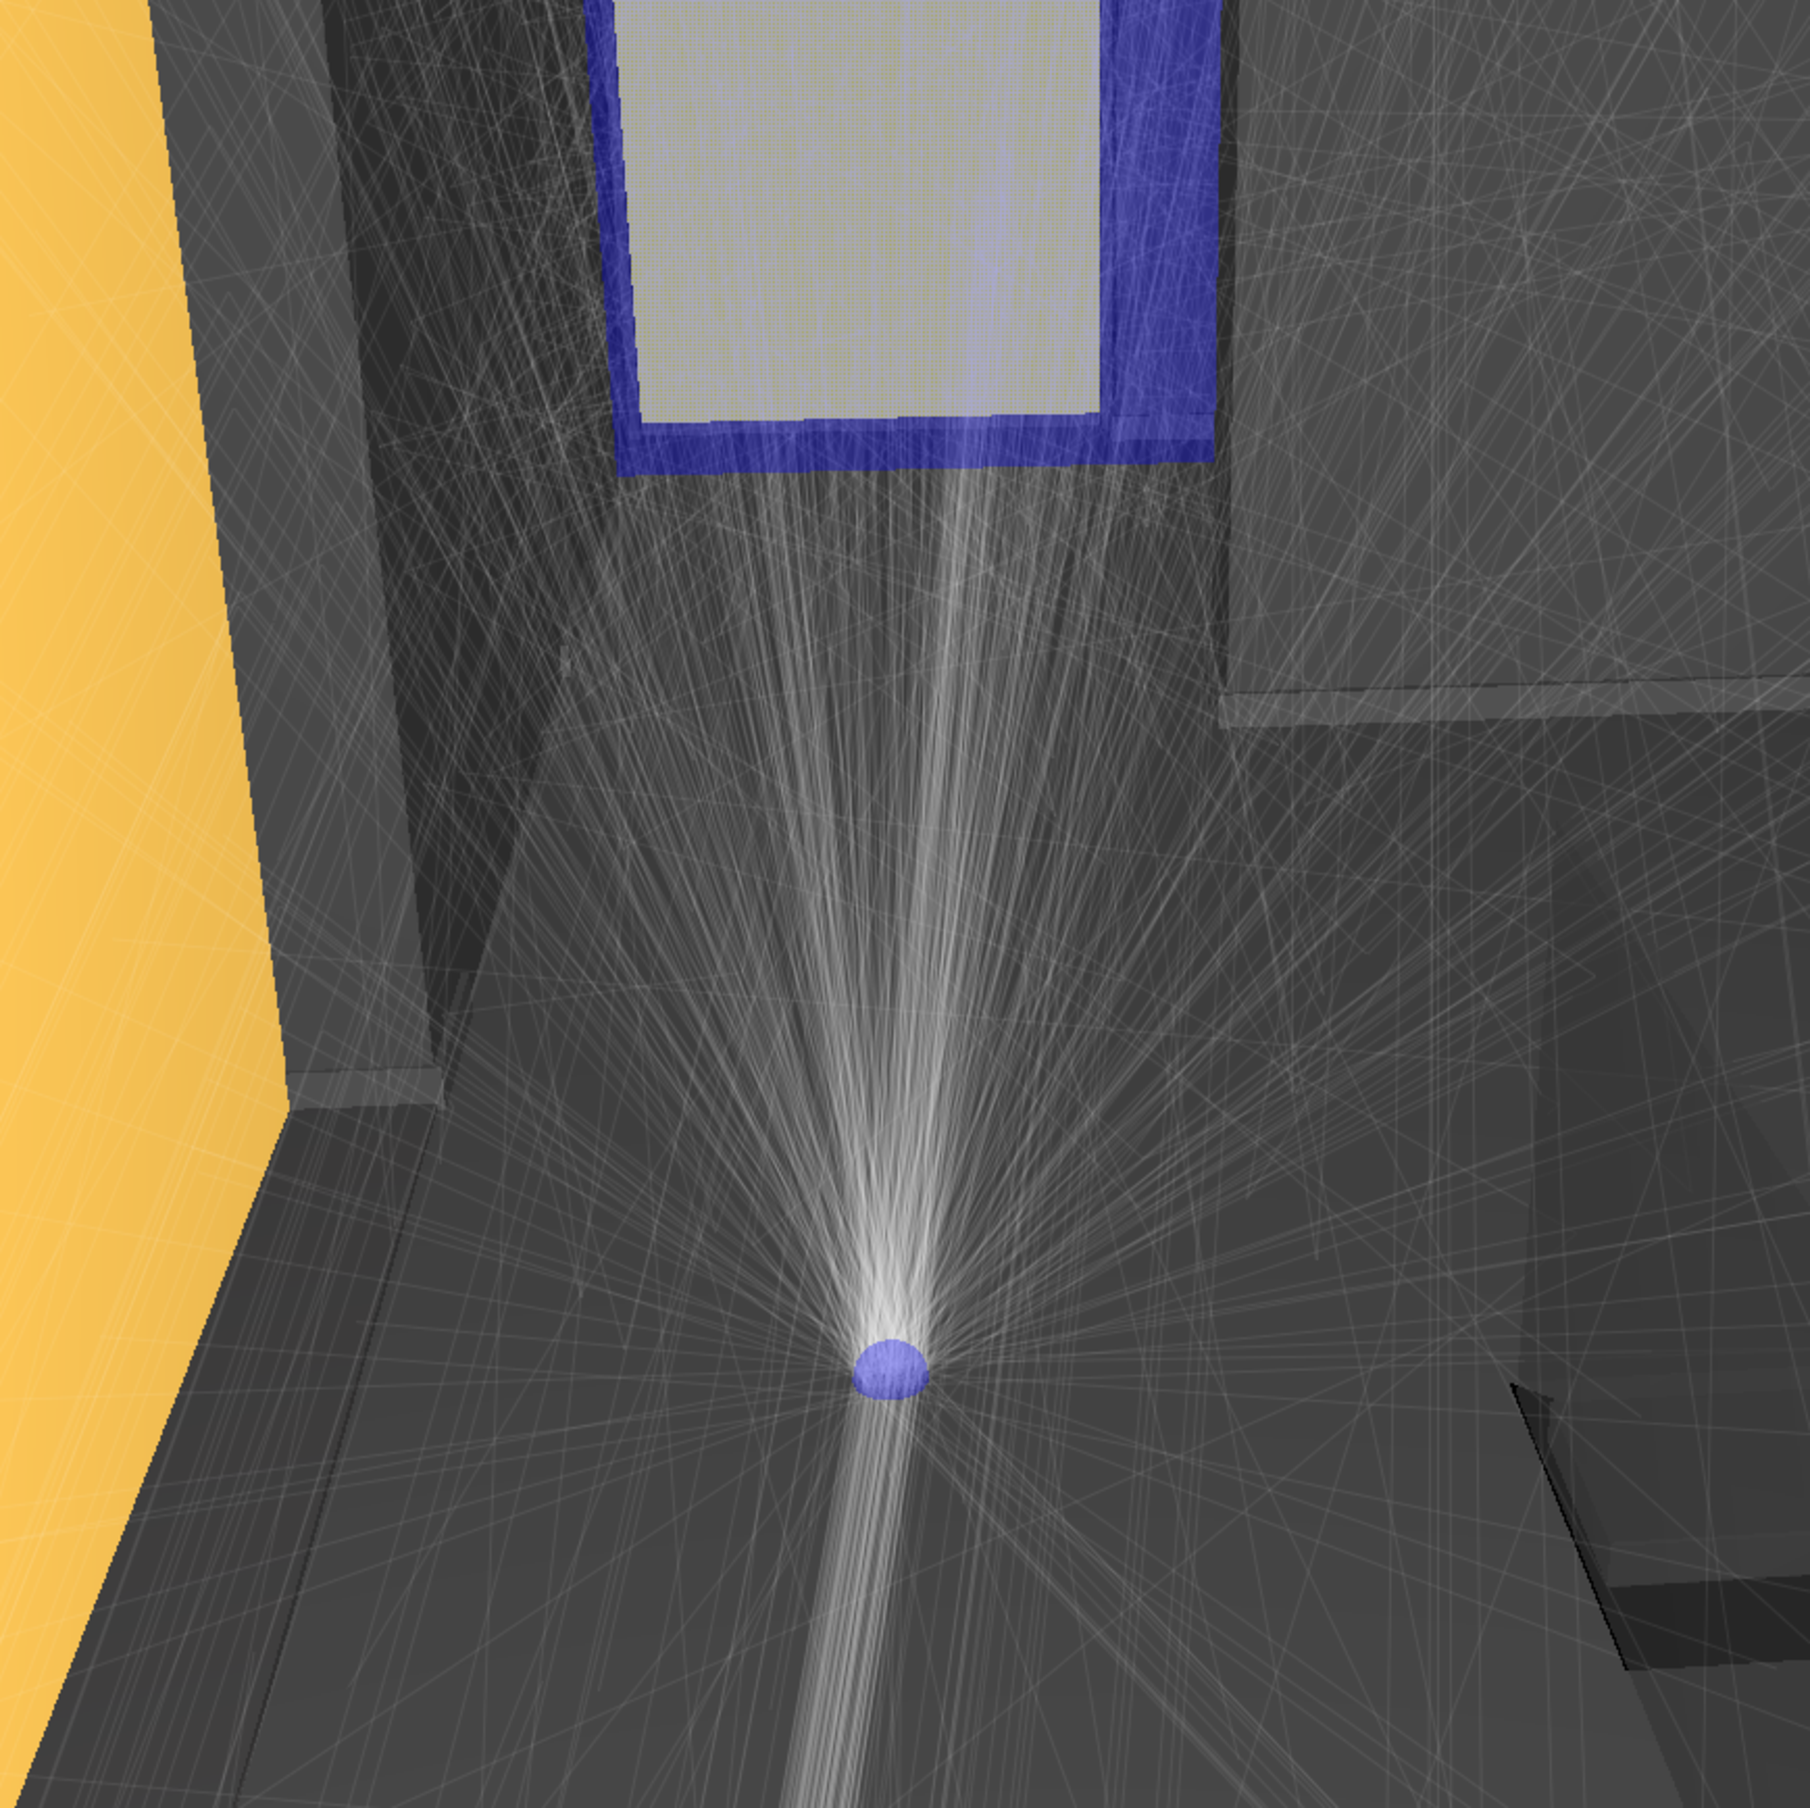
\includegraphics[width=\textwidth]{chapters/chapter_results/correct2paths}
		\caption{\texttt{A}, no radiance scaling}
	\end{subfigure}
	\begin{subfigure}[t]{0.24\linewidth}
		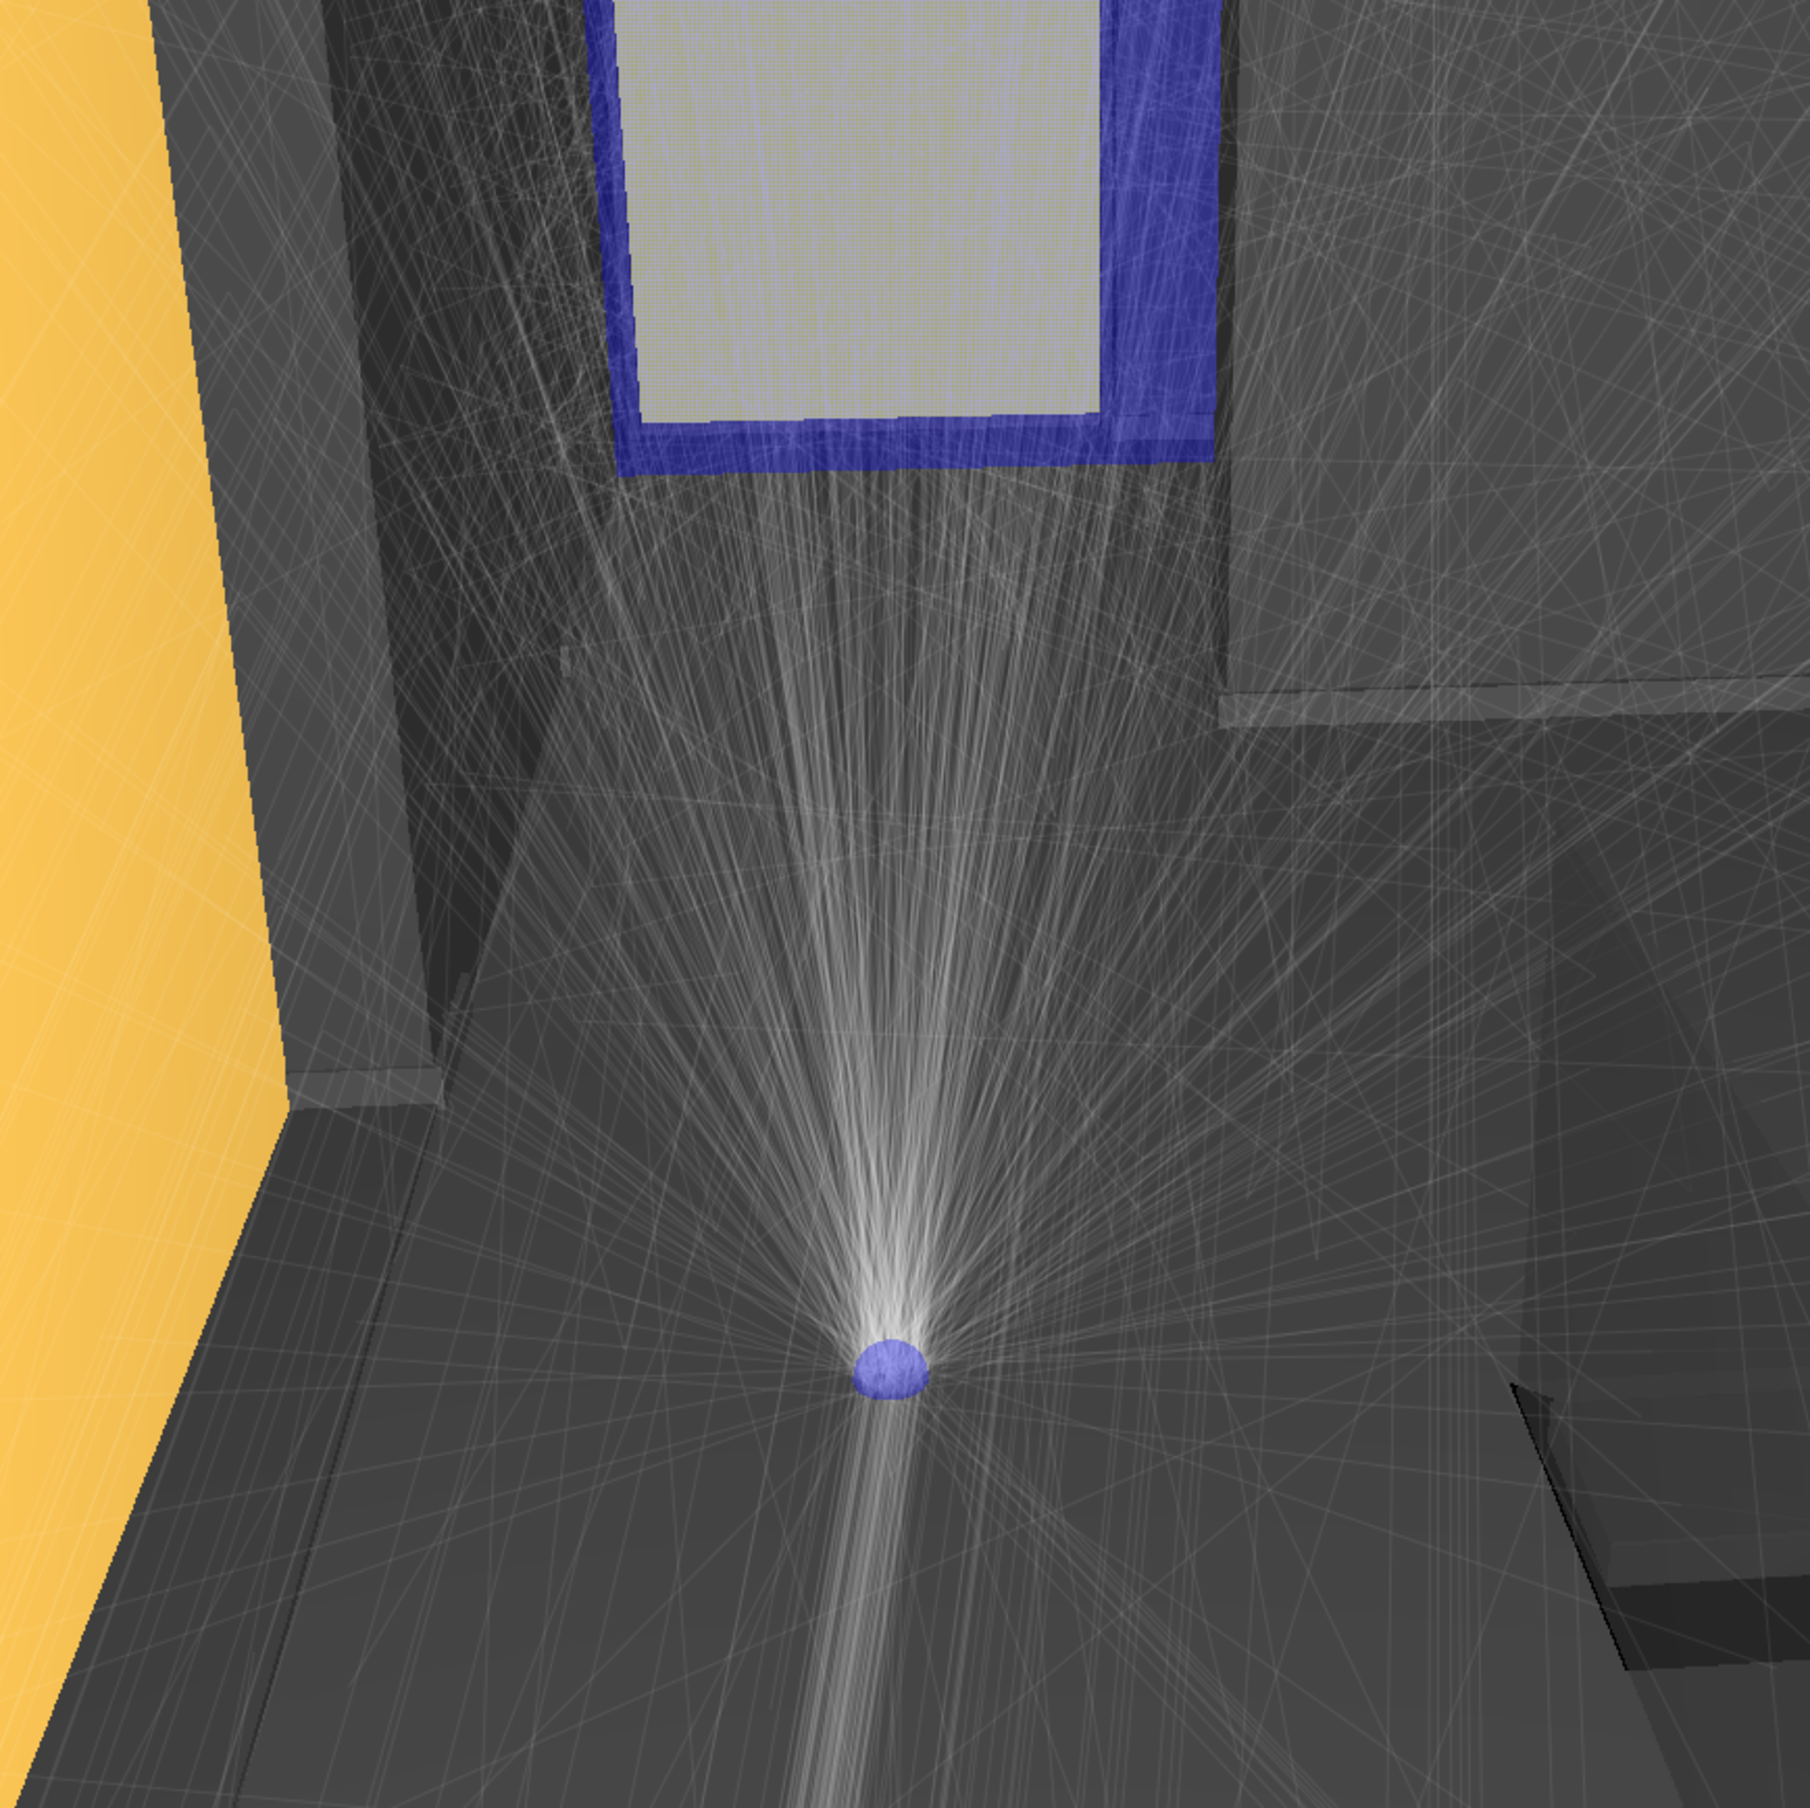
\includegraphics[width=\textwidth]{chapters/chapter_results/wrong2paths}
		\caption{\texttt{B}, no radiance scaling}
	\end{subfigure}

	\caption{Viewport renderings of paths bouncing in the sphere filter placed on the floor and through the window filter on the light in the back. (\textbf{a}) and (\textbf{b}) have the \textbf{“Radiance scaling”} visualization option activated while the others do not. Scene rendering has been darkened using the tool's visualization options.}
	\label{couple2paths}
\end{figure}

It all seemed even further confirmed by placing a sphere filter on the floor where the Fresnel effect shows and analyzing the geometry of paths through there. As shown in figure \ref{couple2paths}, a clear bundle of rays going from the sphere to the window filter appears for dataset \texttt{A}, but not for dataset \texttt{B}. When only looking at those paths having the \textbf{“Radiance scaling”} visualization option activated (fig. \ref{correct2pathsscaled} and \ref{wrong2pathsscaled}), the theory about the error in the Fresnel term computation  might still stand strong; after all, due to the high quantity of paths displayed, it is difficult to understand if that bundle of rays is there in both datasets but it carries way less radiance in dataset \texttt{B} due to miscalculations while evaluating the material.

All doubts are dispelled by disabling the \textbf{“Radiance scaling”}. As soon as it is off, it is clear that that bundle of rays is there, no matter the energy it carries. It shows that the problem is in the picking of a new ray direction that, even if strictly related to surface material evaluation, it is still not in the Fresnel term evaluation.

This conclusion, even if correct, has been drawn by taking several steps in a direction probably dictated by our previous knowledge of the bug. We do not know and cannot make estimates on how any different user would approach the debugging process having this tool available. Nevertheless, this example would fit way more in an educational context as much as the previous did: it could be used to show in a visual way the crucial importance of correct next event estimation since it does not only affect the convergence times --- so how much noise ends up being in the final image --- but also the \textit{correctness} of the render process.